\section{Architectural Design}
\subsection{Overview}
The figure shown below represents a high-level description of the components which make up the System.
The architectural design of the System is divided between eMSP and CPMS. \\
The former describes the part of the System dedicated to offer a Web App for
EV Drivers to plan their charges, book a charge and manage the charges. \\
The latter describes the CPMSs used by the CPOs to manage the reservations, the CP, the energy mix and the contracts with the DSOs.
Both the two parts consists of a four tier architecture that can be grouped into three logical layers: presentation, business logic and data.
\begin {enumerate}
\item Presentation Layer: it manages the presentation logic and all the interactions with the end users
\item Business Logic Layer: it manages the application functions that the S2B provide
\item Data Layer: it manages the safe storage and the access to data
\end{enumerate}
\hfill \\
In this document the presentation layer and the Client (e.g. the Browser)
will be referred to as the Frontend, while the Application Layer and the Data Layer
will be referred to as the Backend.

\begin{figure}[H]
    \centering
    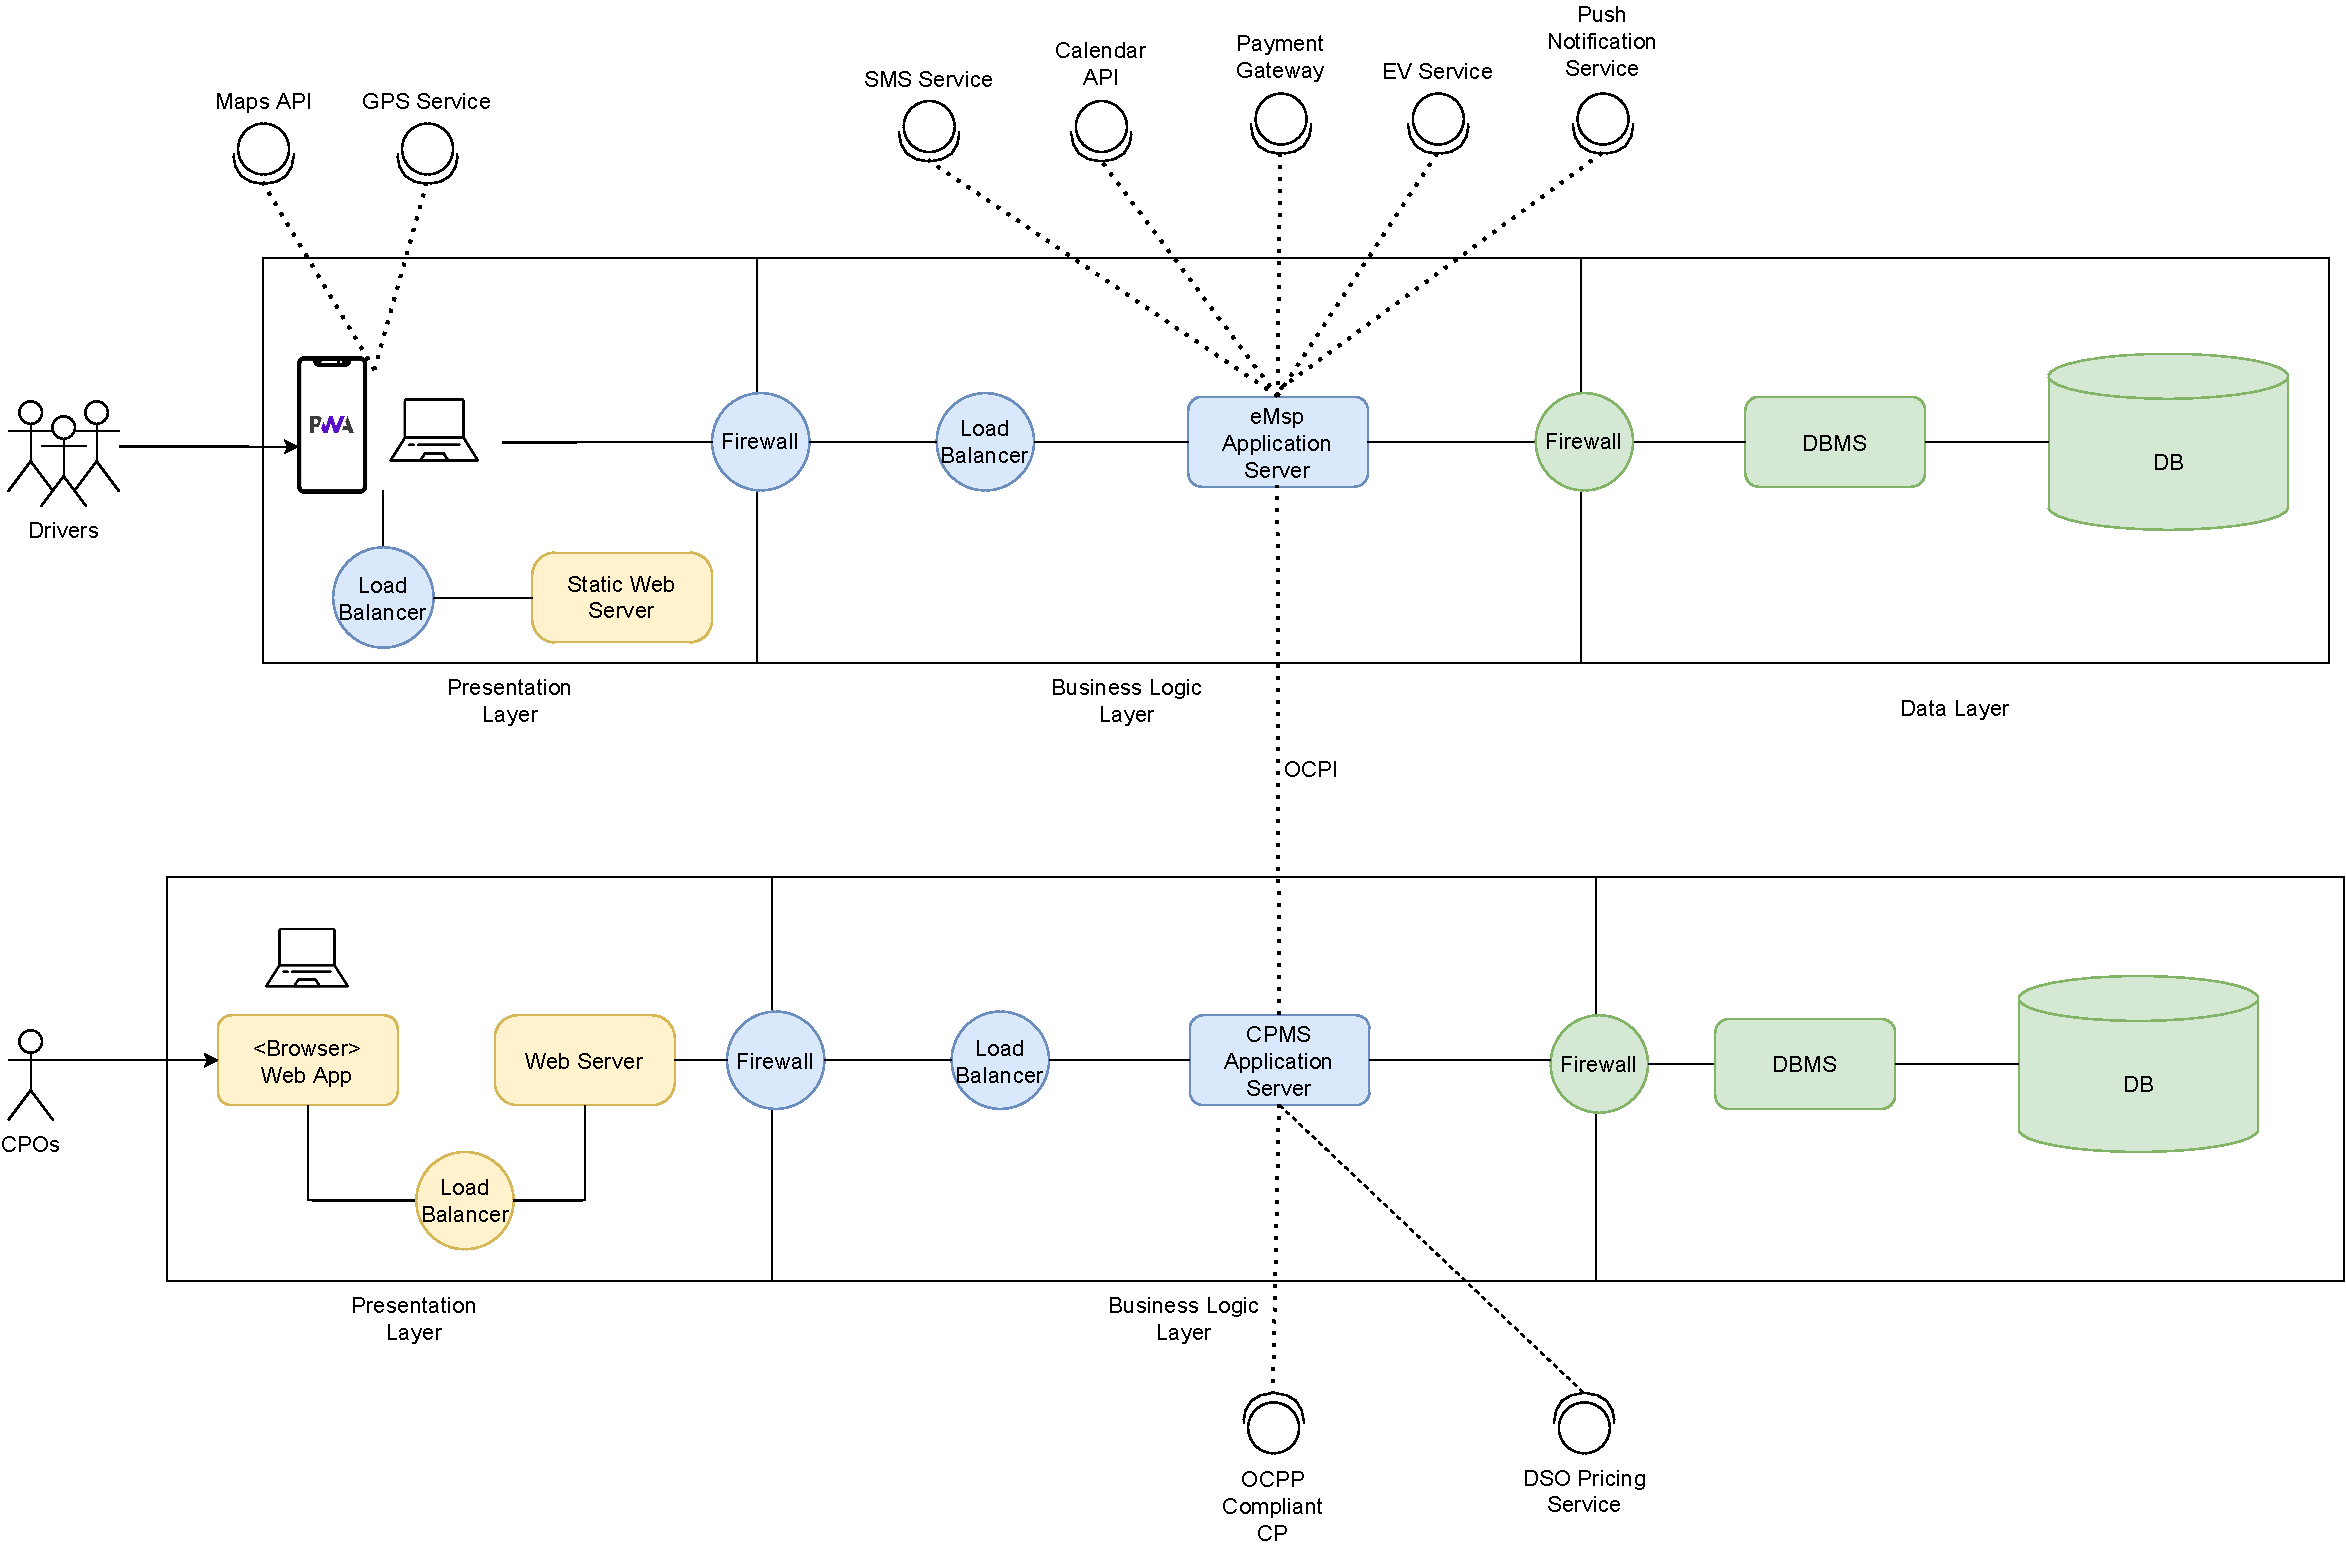
\includegraphics[scale=0.42]{src/Overview/overview_diagram.pdf}
\end{figure}

\hfill \\
The service is supposed to be accessed through a web interface.
Since the features offered and the intensity of the interaction with the application server
are very different depending on the type of user, the web interfaces will be developed following
different principles.
For the EV Drivers an SPA will be developed. An SPA is well-suited for applications
that require a lot of interaction and do not need to perform frequent full page reloads.
They can provide a faster and more seamless user experience for applications that require a
lot of interaction.
For the CPO an SSR Dashboard will be developed. SSR can provide a faster user experience
the server pre-renders the content, reducing the amount of work that the client needs to do.
The Overview Architecture of the S2B divides the application in the layers described
above, and contains some replicated Web Servers, which act as a middleware
between the user's browser and the application servers.
Finally, the application servers interfaces with the DBMS APIs, in order
to retrieve and store the data required for the considered computation.
The applications servers are expected to be stateless, according to the
REST standard definitions. The nodes are separated by firewalls to guarantee a higher level of security
of the whole system.

\begin{itemize}
    \item Static Web Server: it does not execute any business logic, but simply receive requests from the client and serve an HTML file along with other static assets (CSS Sheets, JS files, \dots).
          It does not route the request to the Application Server
    \item Web Server: it does not execute any business logic, but simply receive requests from the client, route
          them to the application servers which build the HTML page (along with the static assets) and send it back to the web server which serve the client
\end{itemize}
\pagebreak
\subsection{Component view}
In this section we show the components of the S2B, their relationships and interfaces. The following sections will explain the interaction between interfaces and details on each method of interfaces with REST endpoints, if any.

\begin{figure}[H]
    \centering
    \hspace*{-2cm}
    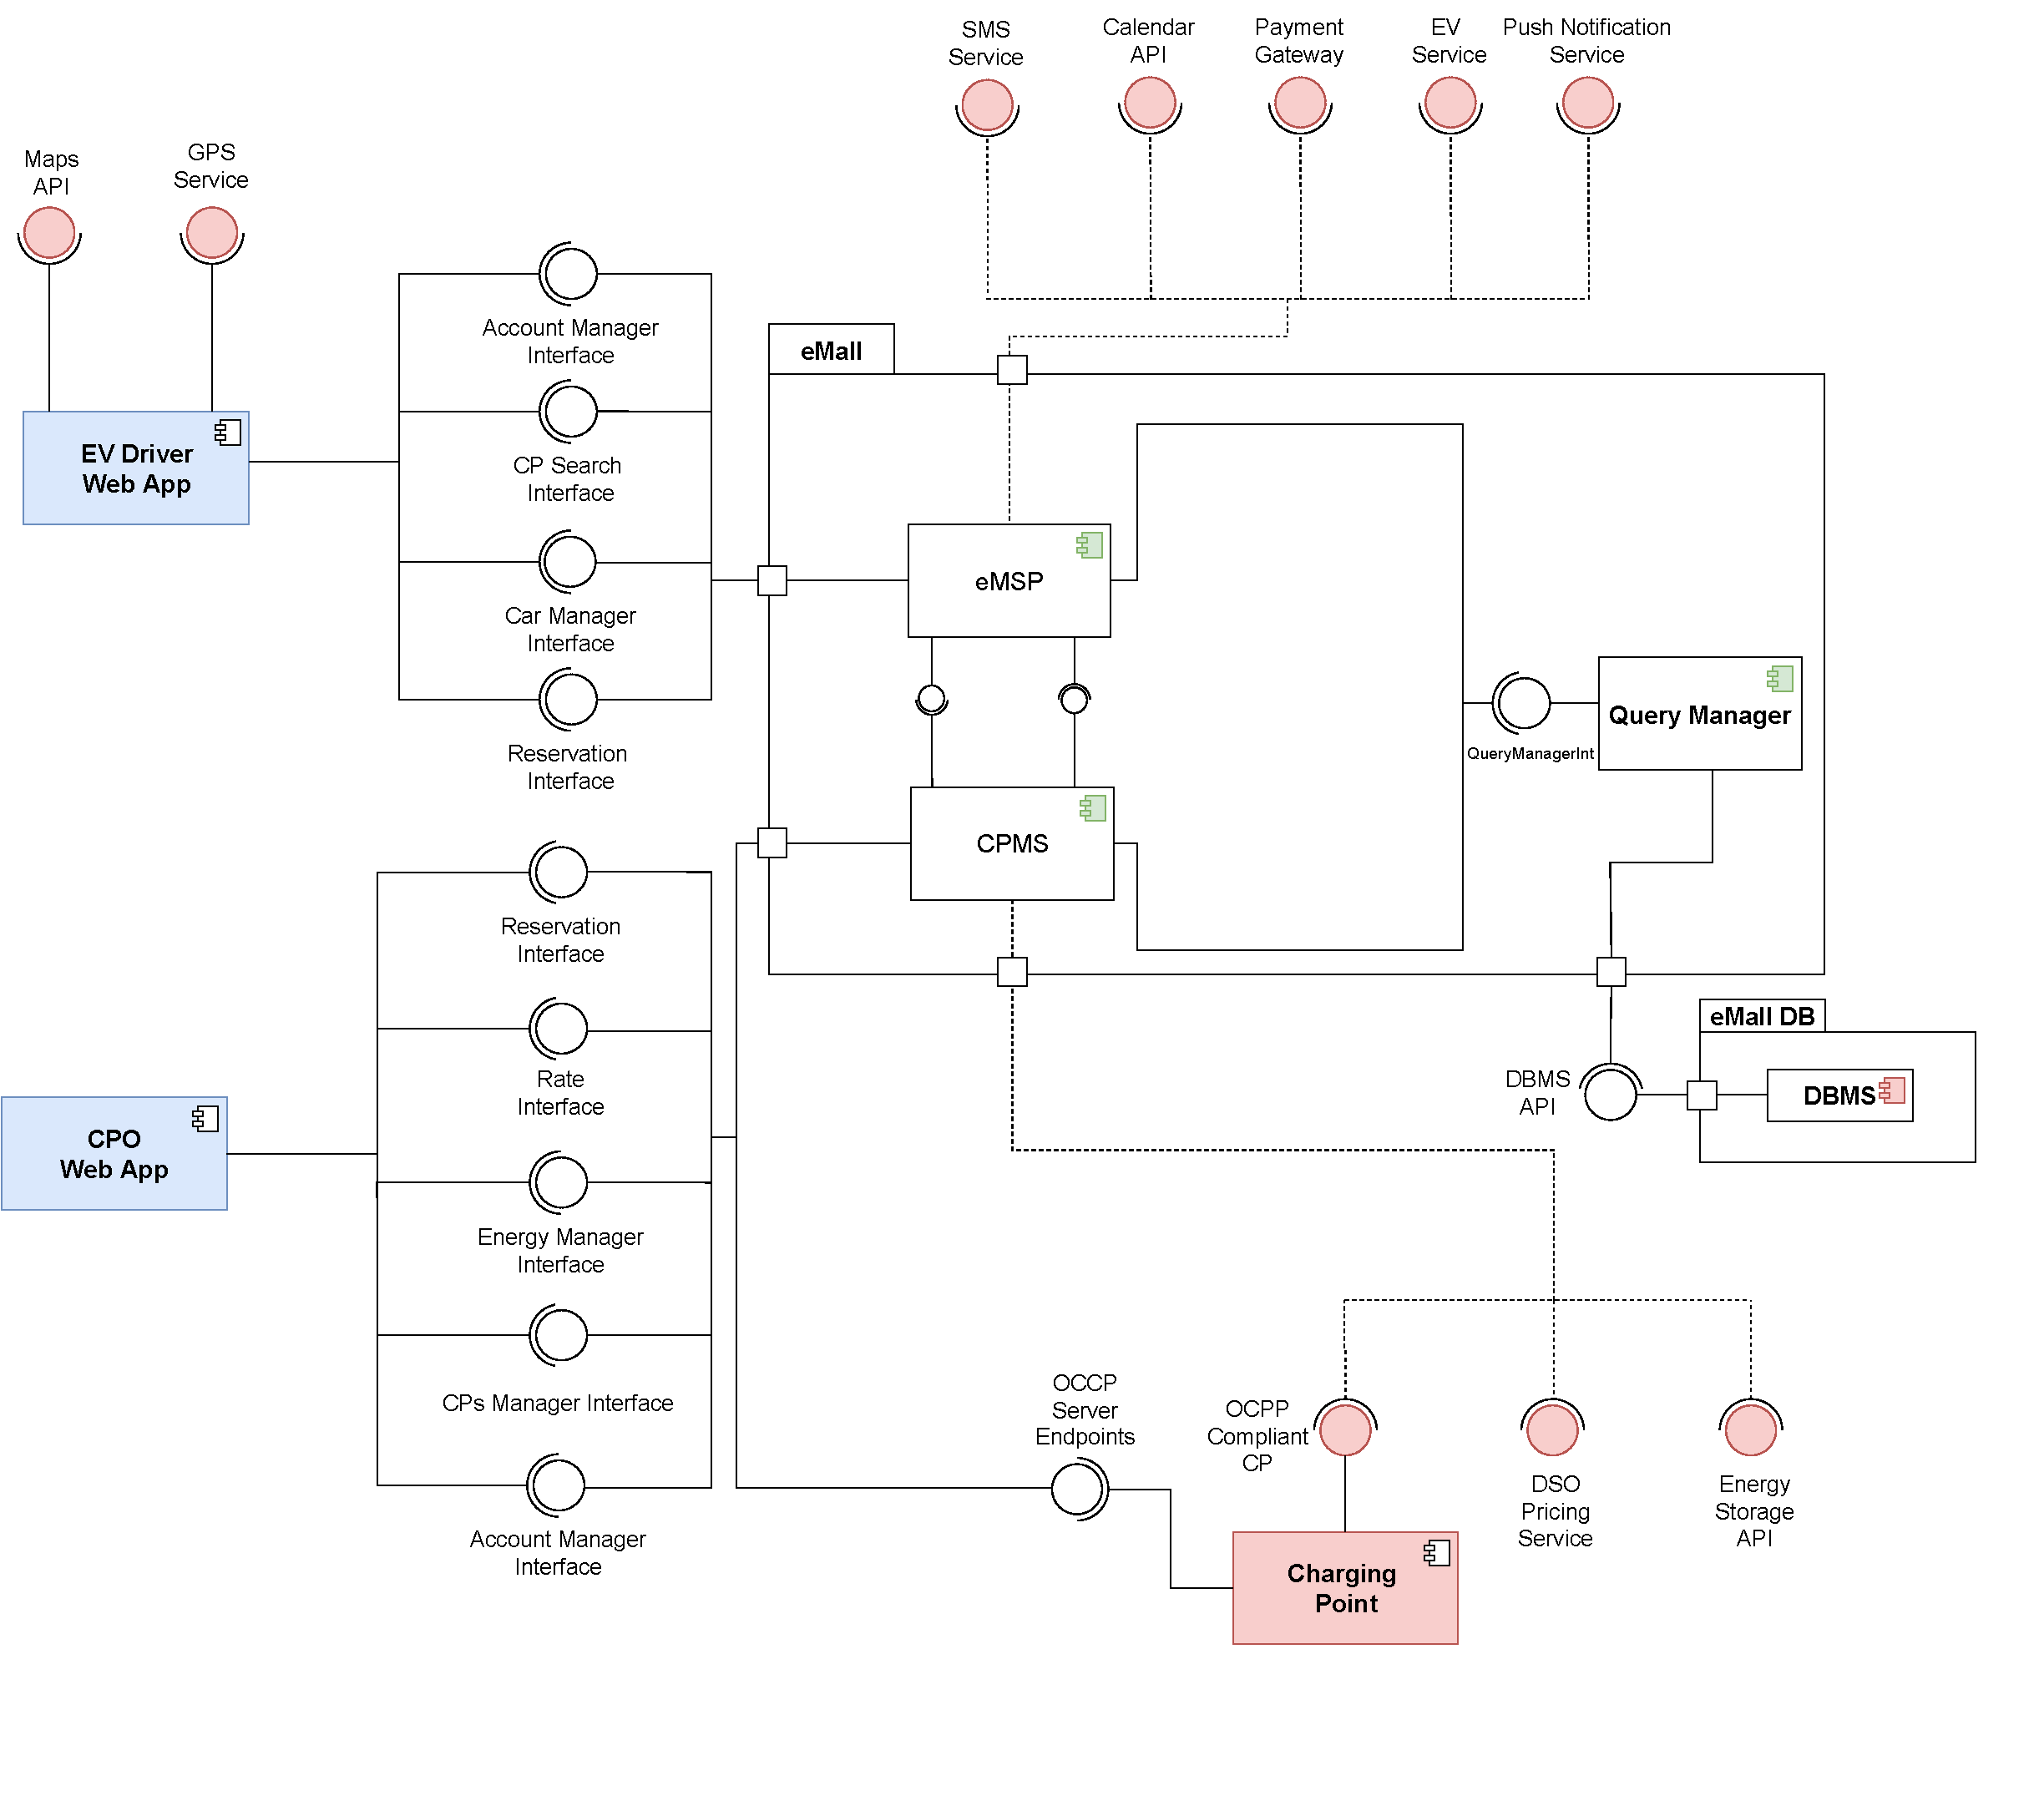
\includegraphics[scale=0.5]{src/ComponentDiagram/overview_component_diagram.pdf}
    \caption{Component Diagram of the eMall System}
\end{figure}


\subsubsection{eMSP}

\begin{figure}[H]
    \centering
    \hspace*{-2cm}
    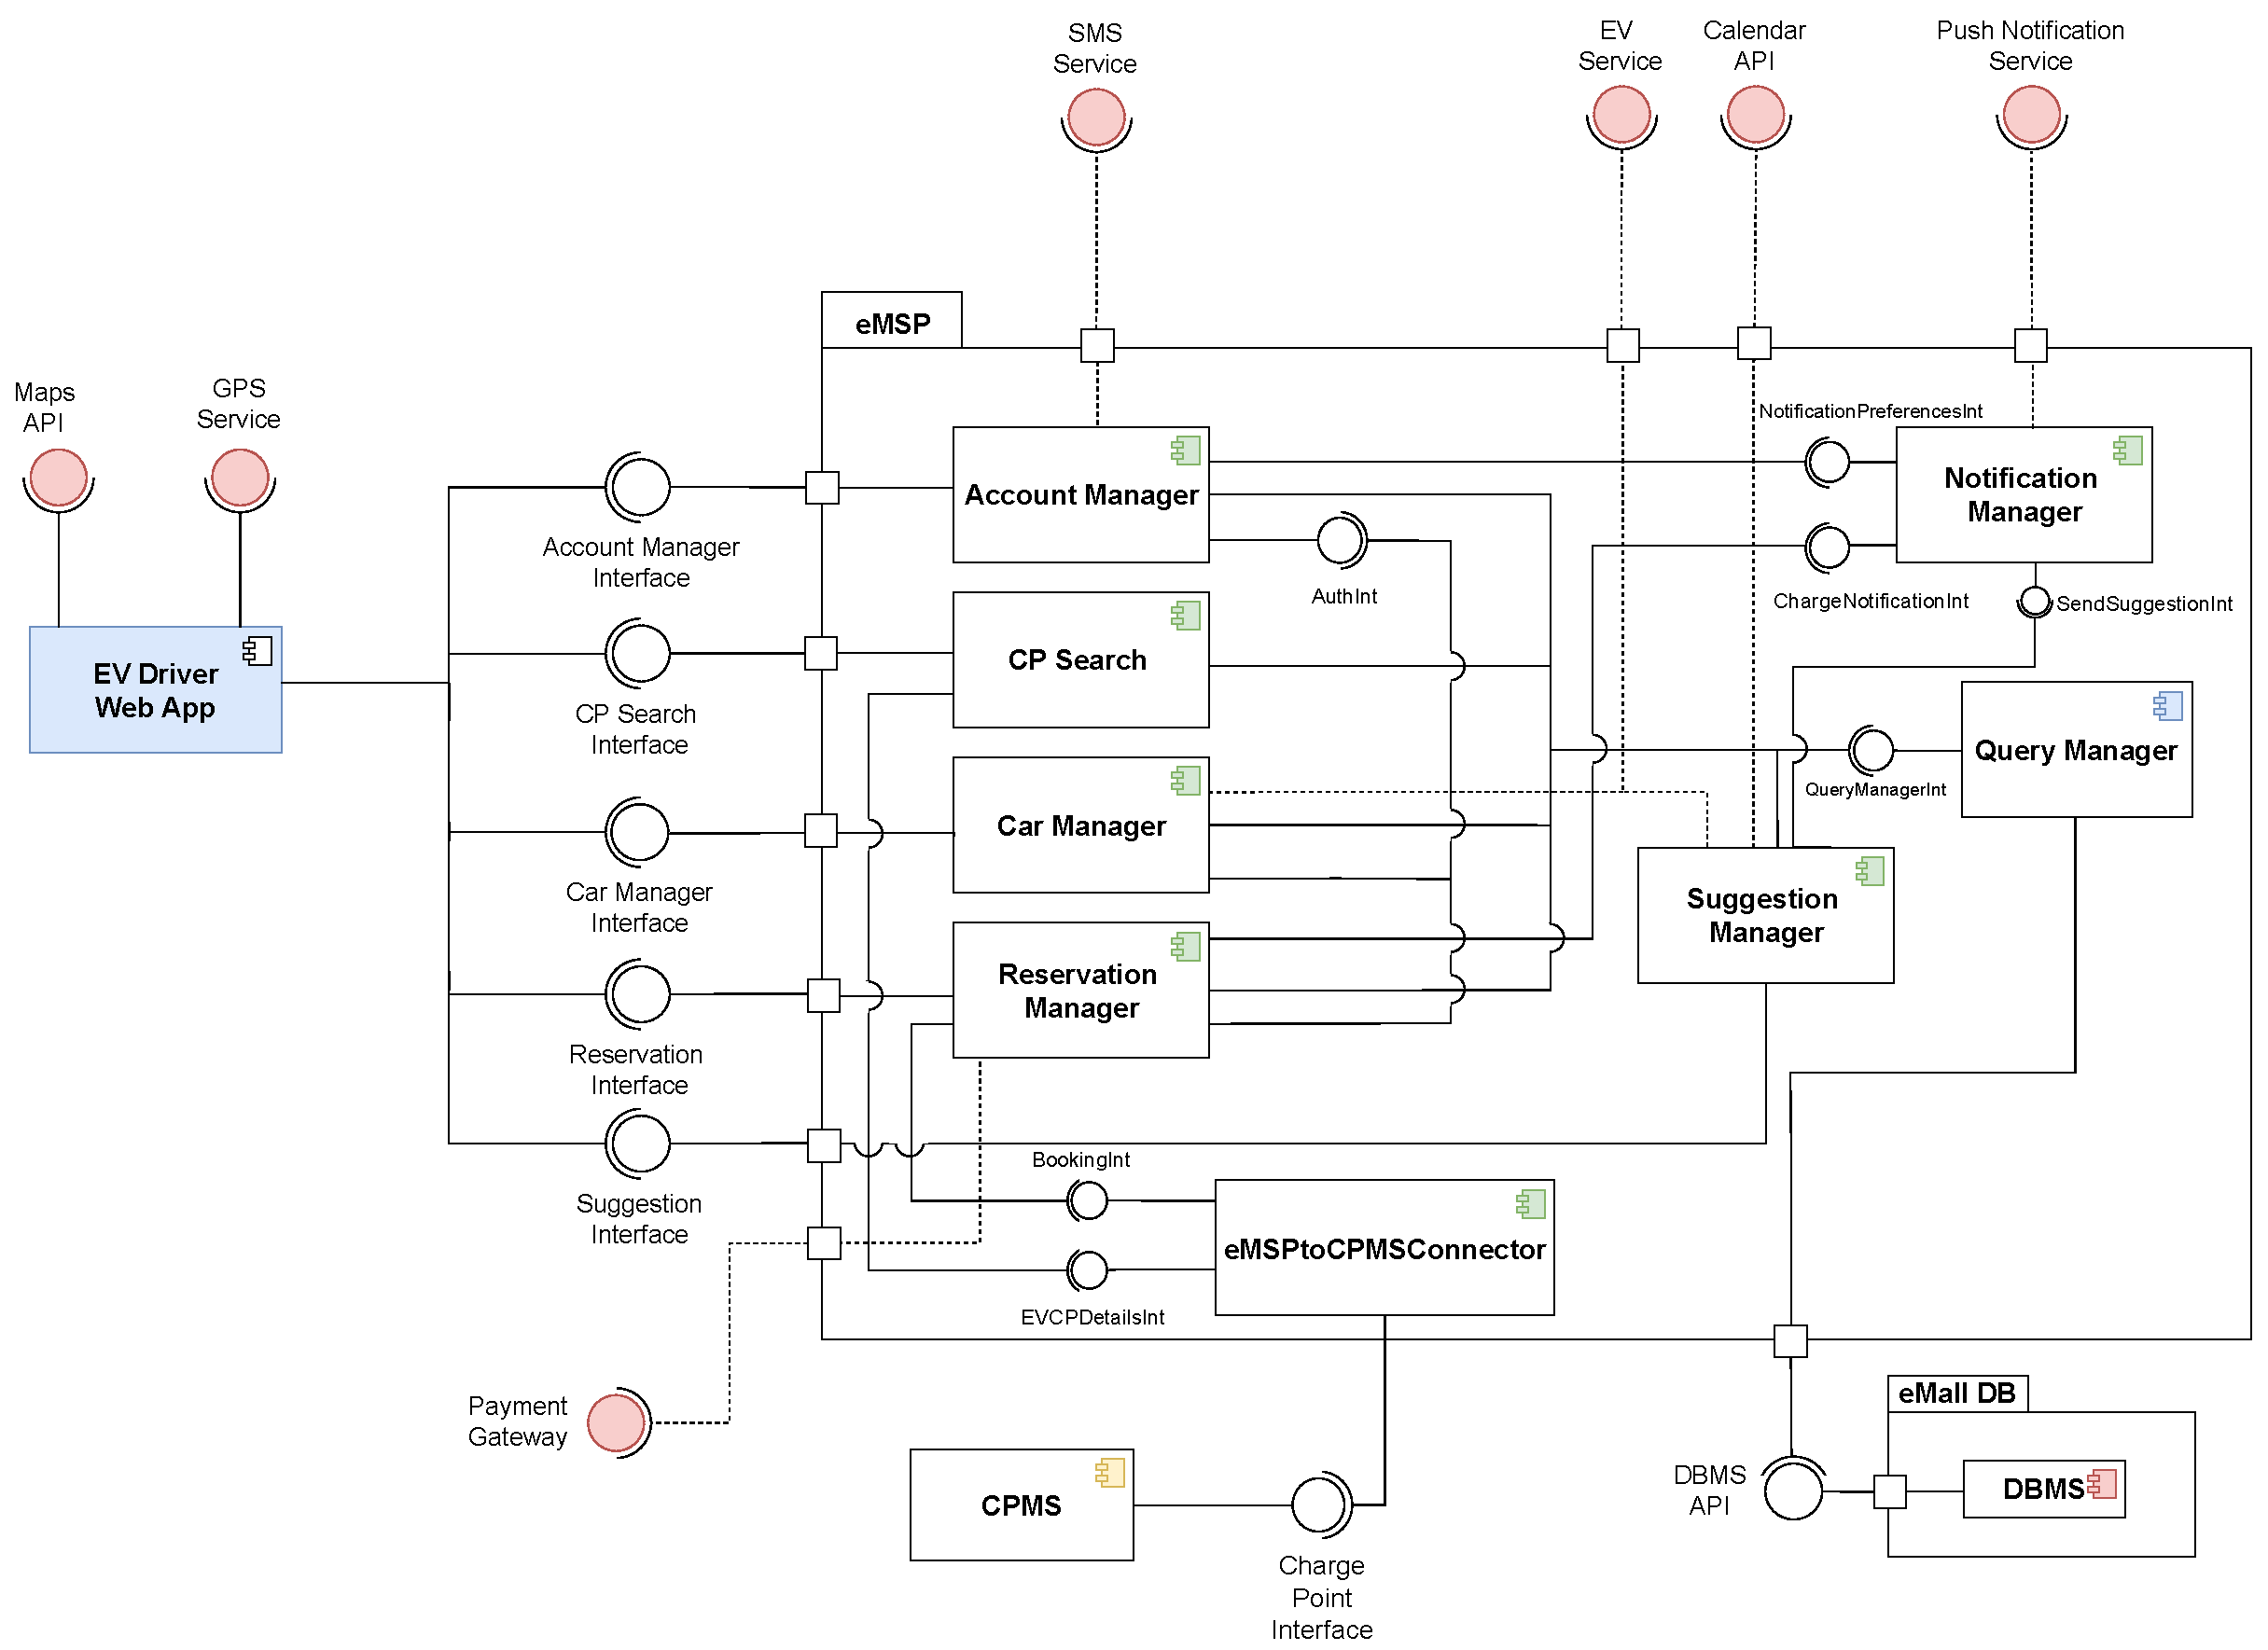
\includegraphics[scale=0.5]{src/ComponentDiagram/emsp_component_diagram.pdf}
    \caption{Component Diagram of the eMSP subsystem}
\end{figure}

\paragraph*{eMSP Web App} \hfill \\
It represents the application dedicated to the EV drivers. This component uses client side rendering of web pages. 
The user through the browser sends a request to the server and the eMSP Application Server responds with the HTML and Javascript which the browser then
downloads and execute. As the user interacts with the page, the Javascript can make additional requests to the server and update
the page dynamically, without need to fully reload the page. 
\paragraph*{eMSP Application Server} \hfill \\
The eMSP Application Server is responsible for the business logic to provide the functionality to the application for the EV Drivers and to coordinate the information flow between application layer and data layer
It is composed of several components, each of them used for a specific functionality:\\
\begin{itemize}
    \item \textbf{Account Manager} \\ This component handles all the account operations related to the CPO and offers an interface to authenticate
          the requests in the CPMS application server.
          It offers functionality to create new account, logging in, setting preferences and verify the authentication of the user at any time.
          To create a new account interacts with the external SMS API to make the user receive a code to verify the identity.
    \item \textbf{CP Search} \\ This component handles the operations needed to show the CPs in a specified range of km near a location. The location
        can be described as an address, with coordinates or by geolocating the actual position of the incoming request. It selects the filtered CPs that are then 
        shown in the map as placeholders.  
    \item \textbf{Car Manager} \\ This component handles the operations related to the status of the car. It offers an interface to select the EV model among a list of 
        all the marketed models and offers an interface to connect the car to the application. It uses these information to show the battery status of the EV, the 
        amount of power during a charging process and to suggest charging plans based on the specific vehicle and status of it.
    \item \textbf{Reservation Manager} \\ This component handles all the operations related to the reservations for the EV Drivers. It offers the possibility to create a reservation
    for a charge and pay for that reservation, see the details of a reservation, start or pause a charge of a particular reservation and see the recap of an already occurred reservation.
    It permits to pay for a reservation using an external Payment Gateway that handles all the payment process and returns the status of the payment.  

\end{itemize}


\subsubsection{CPMS}

\begin{figure}[H]
    \centering
    \hspace*{-2cm}
    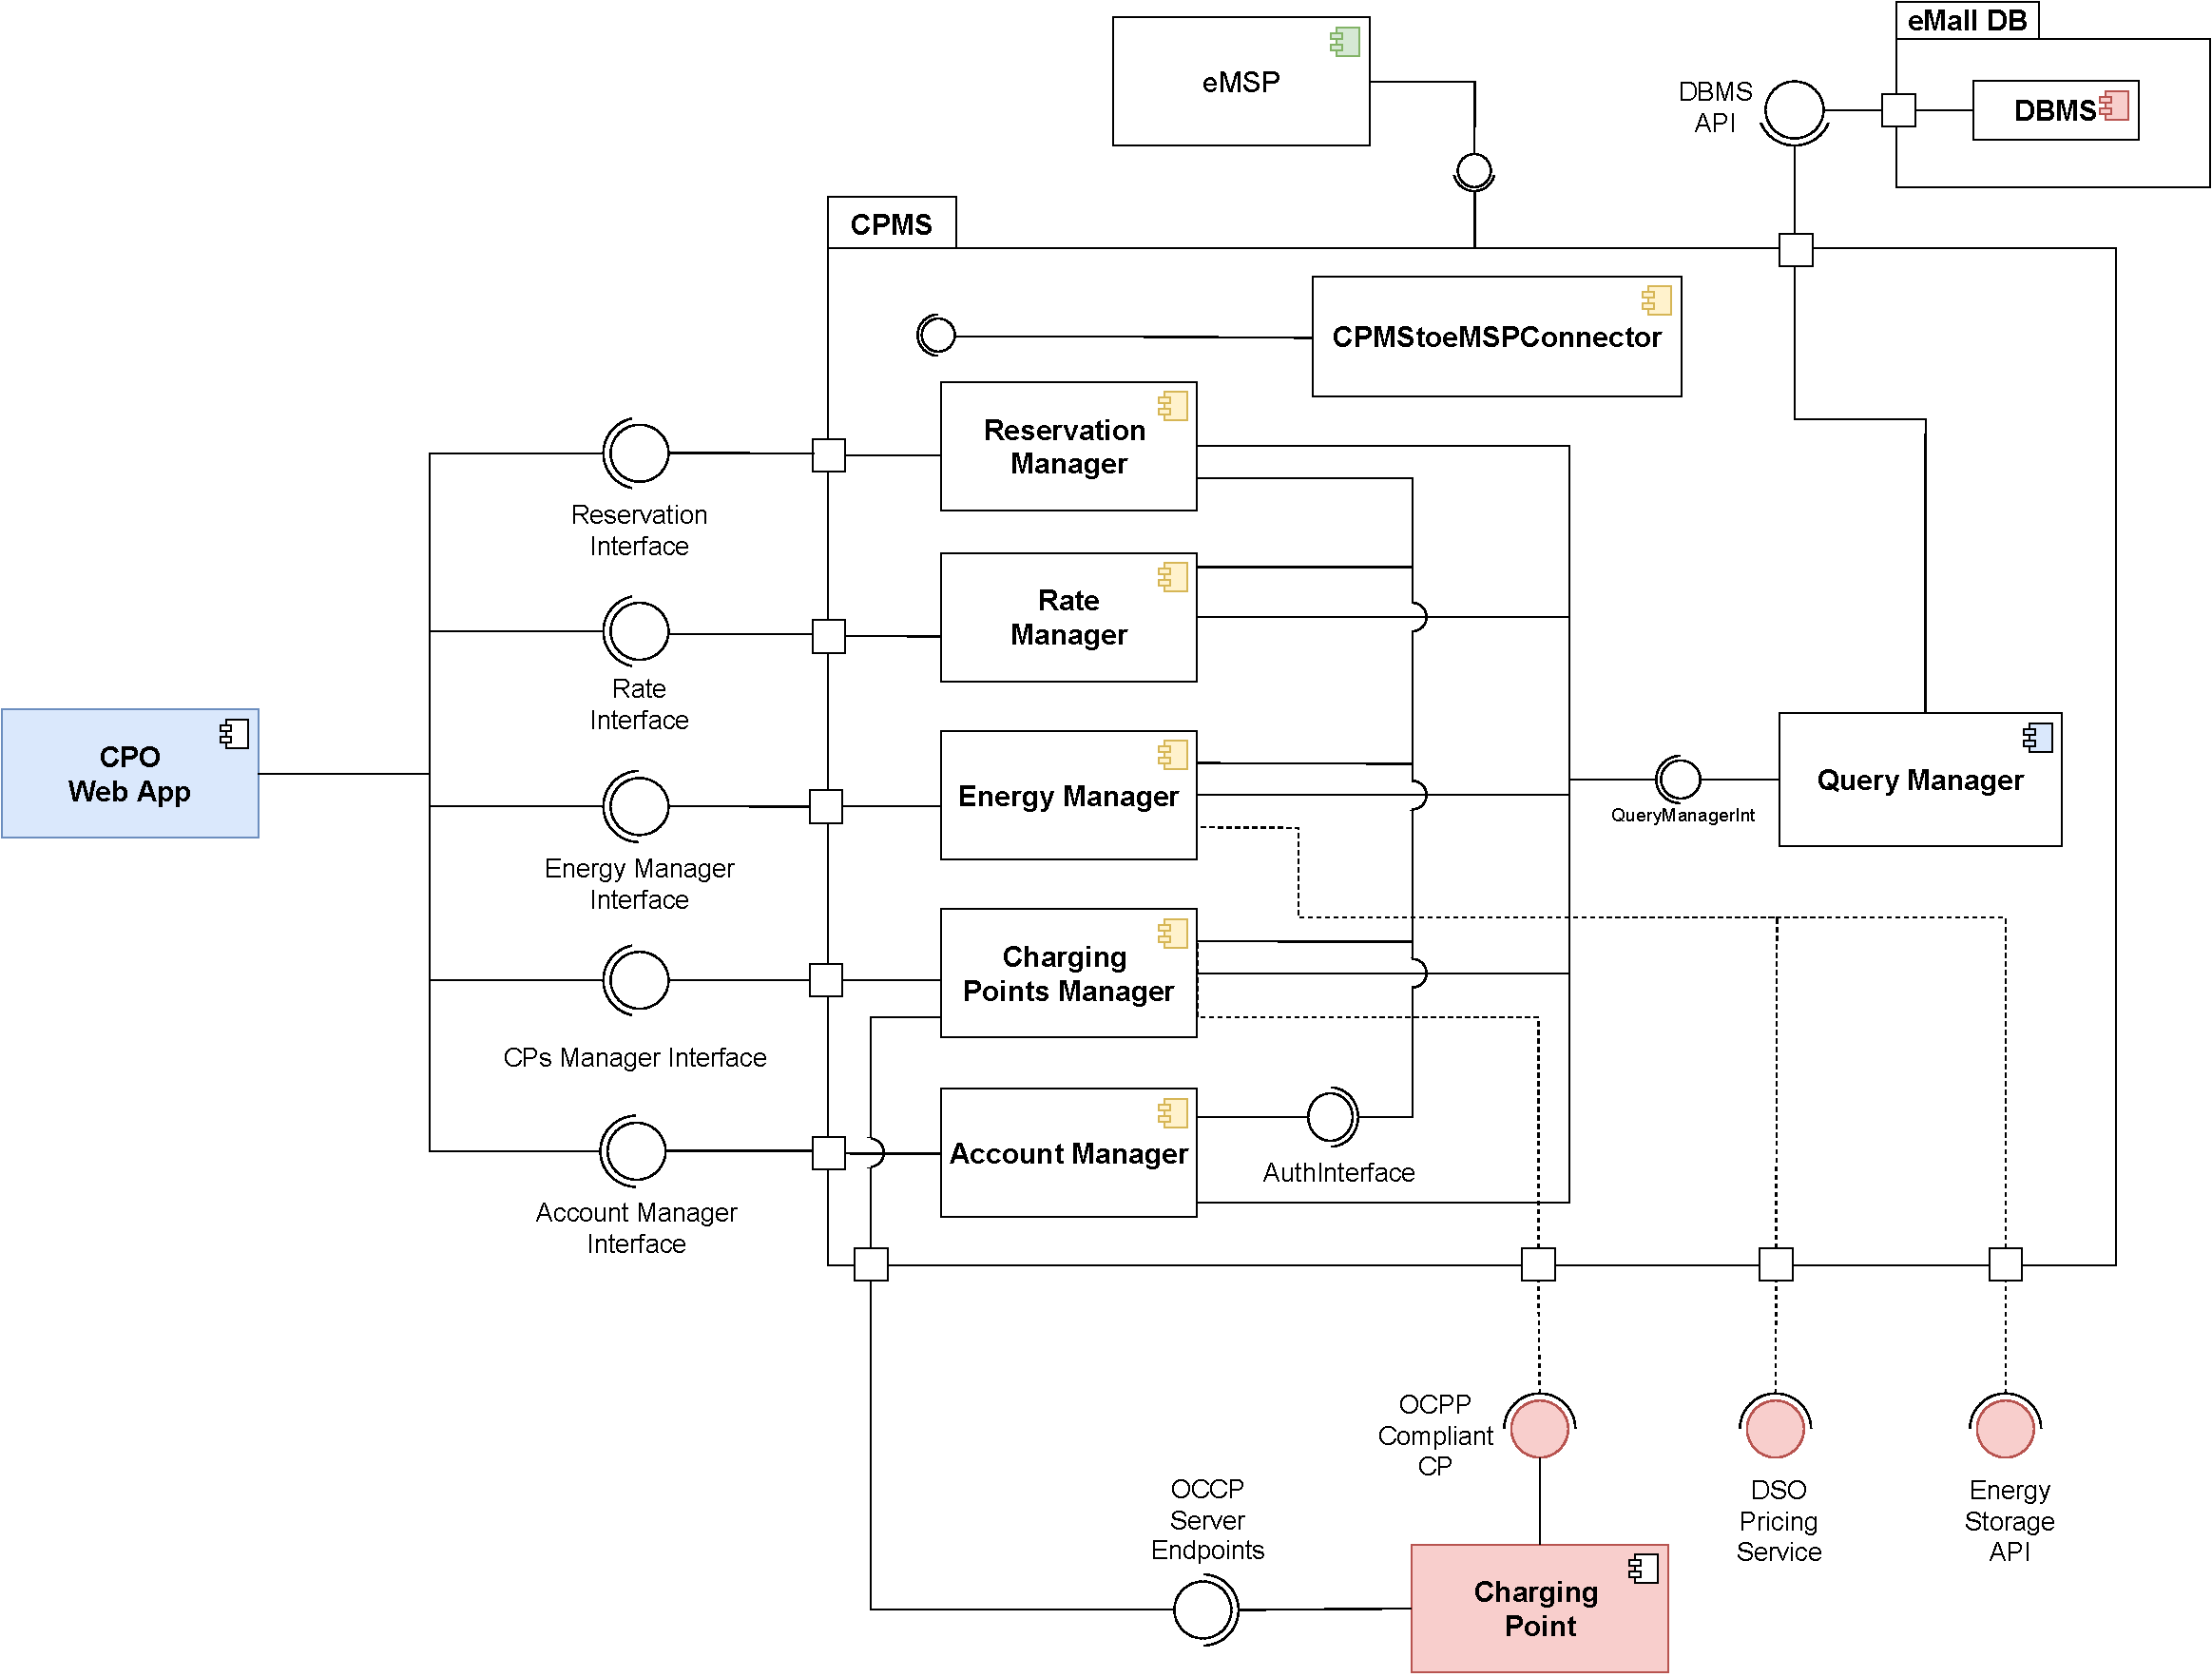
\includegraphics[scale=0.5]{src/ComponentDiagram/cpms_component_diagram.pdf}
    \caption{Component Diagram of the CPMS subsystem}
\end{figure}

\paragraph*{CPO Web App} \hfill \\
It represents the application dedicated to the different CPOs using the system. This component contains the logic to receive HTTPS requests from the users' browser,
forward them to the CPMS Application Server, and generate dynamic pages based on the response from the CPMS Application Server.

\paragraph*{CPMS Application Server} \hfill \\
The CPMS Application Server is responsible for the business logic to provide the functionality to the application for the CPOs and to coordinate the information flow between application layer and data layer.
It is composed of several components, each of them used for a specific functionality:\\
\begin{itemize}
    \item \textbf{Booking Manager} \\
    This component handles the operations regarding the reservation of a specific CPO. It offers the possibility to manage the reservations and to control their status.
    \item \textbf{Rate Manager} \\ This component is responsible for the operations regarding the rates of that are associated with the CPs. It offers the possibility to
    create a new rate in all its details, to add a special rate and specify the duration. The created rates then are associated to a specific CP.
    \item \textbf{Energy Manager} \\ This component is responsible for the operations regarding the managing of the energy of the different EVCPs. 
    It offers the possibility to verify the energy consumption and production of the different sources, modify and visualize the status of the energy storage system,
    visualize the availability of energy contracts provided by the DSOs for a specific EVCP and stipulate a contract among the ones available.
    \item \textbf{Charging Points Manager} \\ This component handles the operations regarding the managing of the CPs. It is an OCPP server for the CPs, offering the 
    required functionalities for adding and removing a CP, for starting and stopping a charge and for receiving status data by the CP. It offers an interface to connect the different CPs through their platform.
    \item \textbf{Account Manager} \\ This component handles all the account operations related to the CPO and offers an interface to authenticate the requests in the CPMS application server.
          It offers functionality to create new account, logging in, setting preferences and verify the authentication of the user at any time.
          To create a new account interacts with the external SMS API to make the user receive a code to verify the identity.
\end{itemize}

\begin{figure}[H]
    \centering
    \hspace*{-2.5cm}
    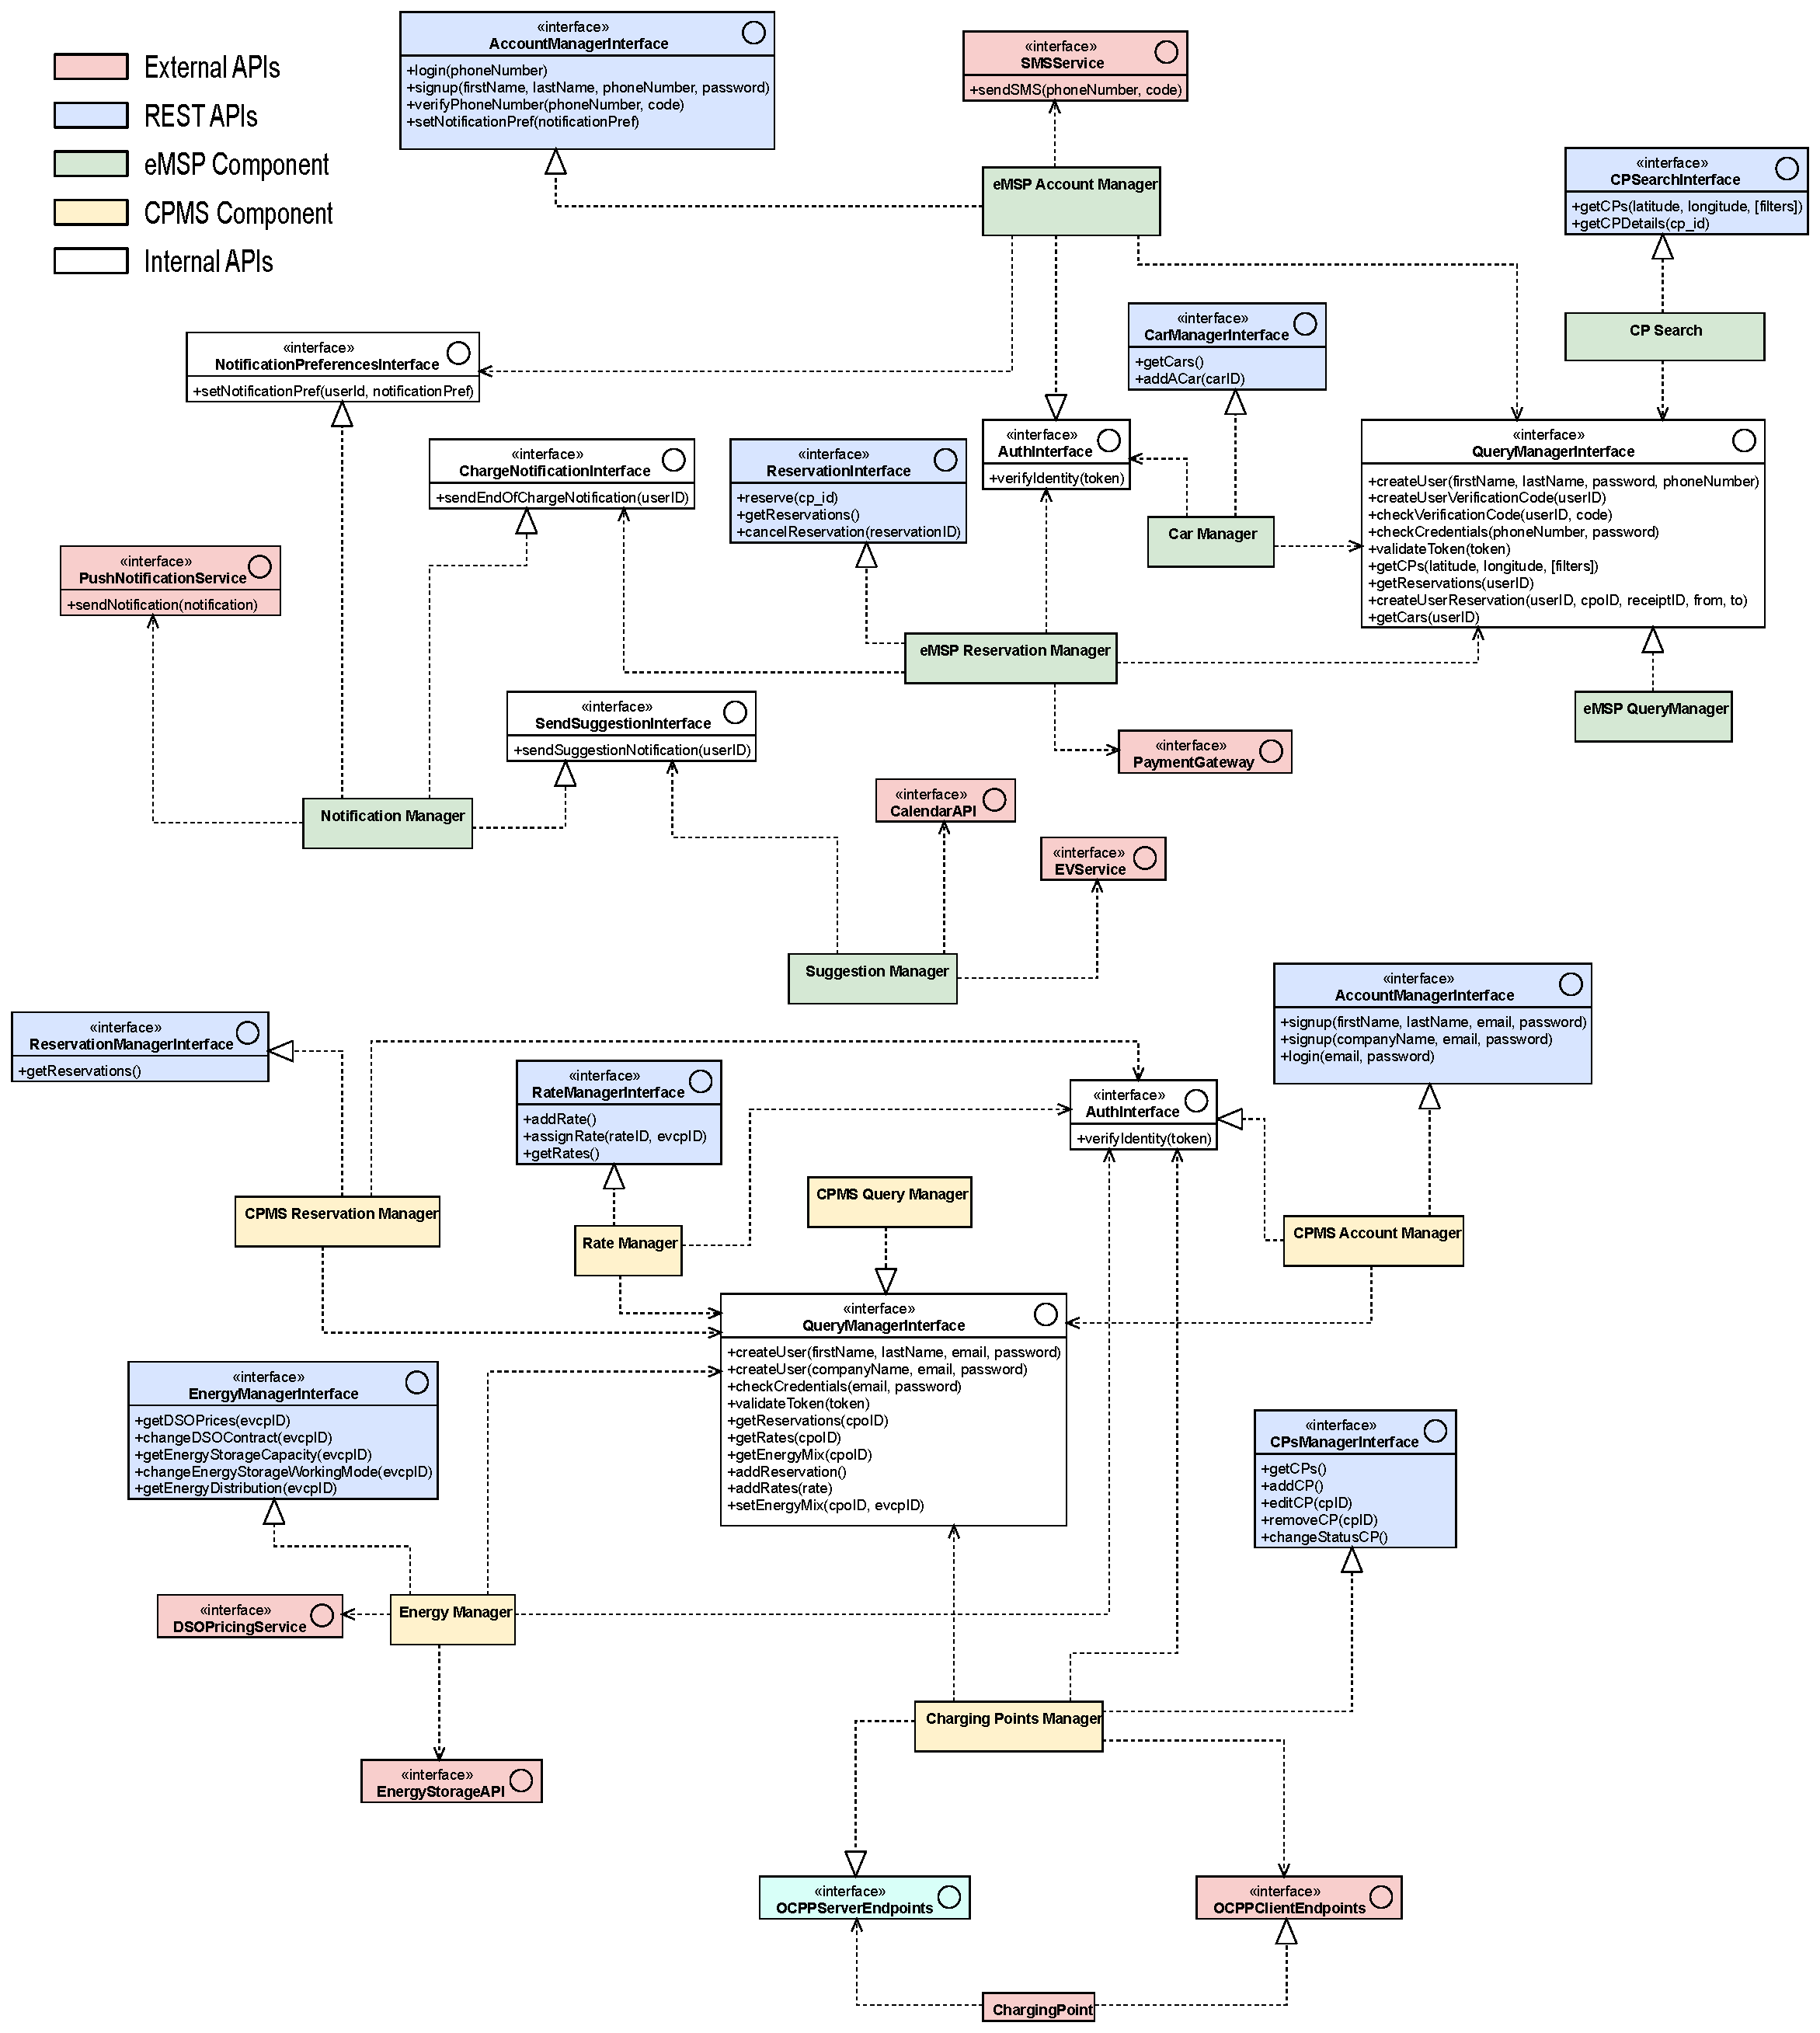
\includegraphics[height=\textheight-1.5cm,keepaspectratio]{src/componentInterfaces/component_interface.pdf}
    \caption{Class Diagram with interfaces of the eMall System}
\end{figure}


\subsubsection{Logical Description of Data}
\begin{figure}[H]
    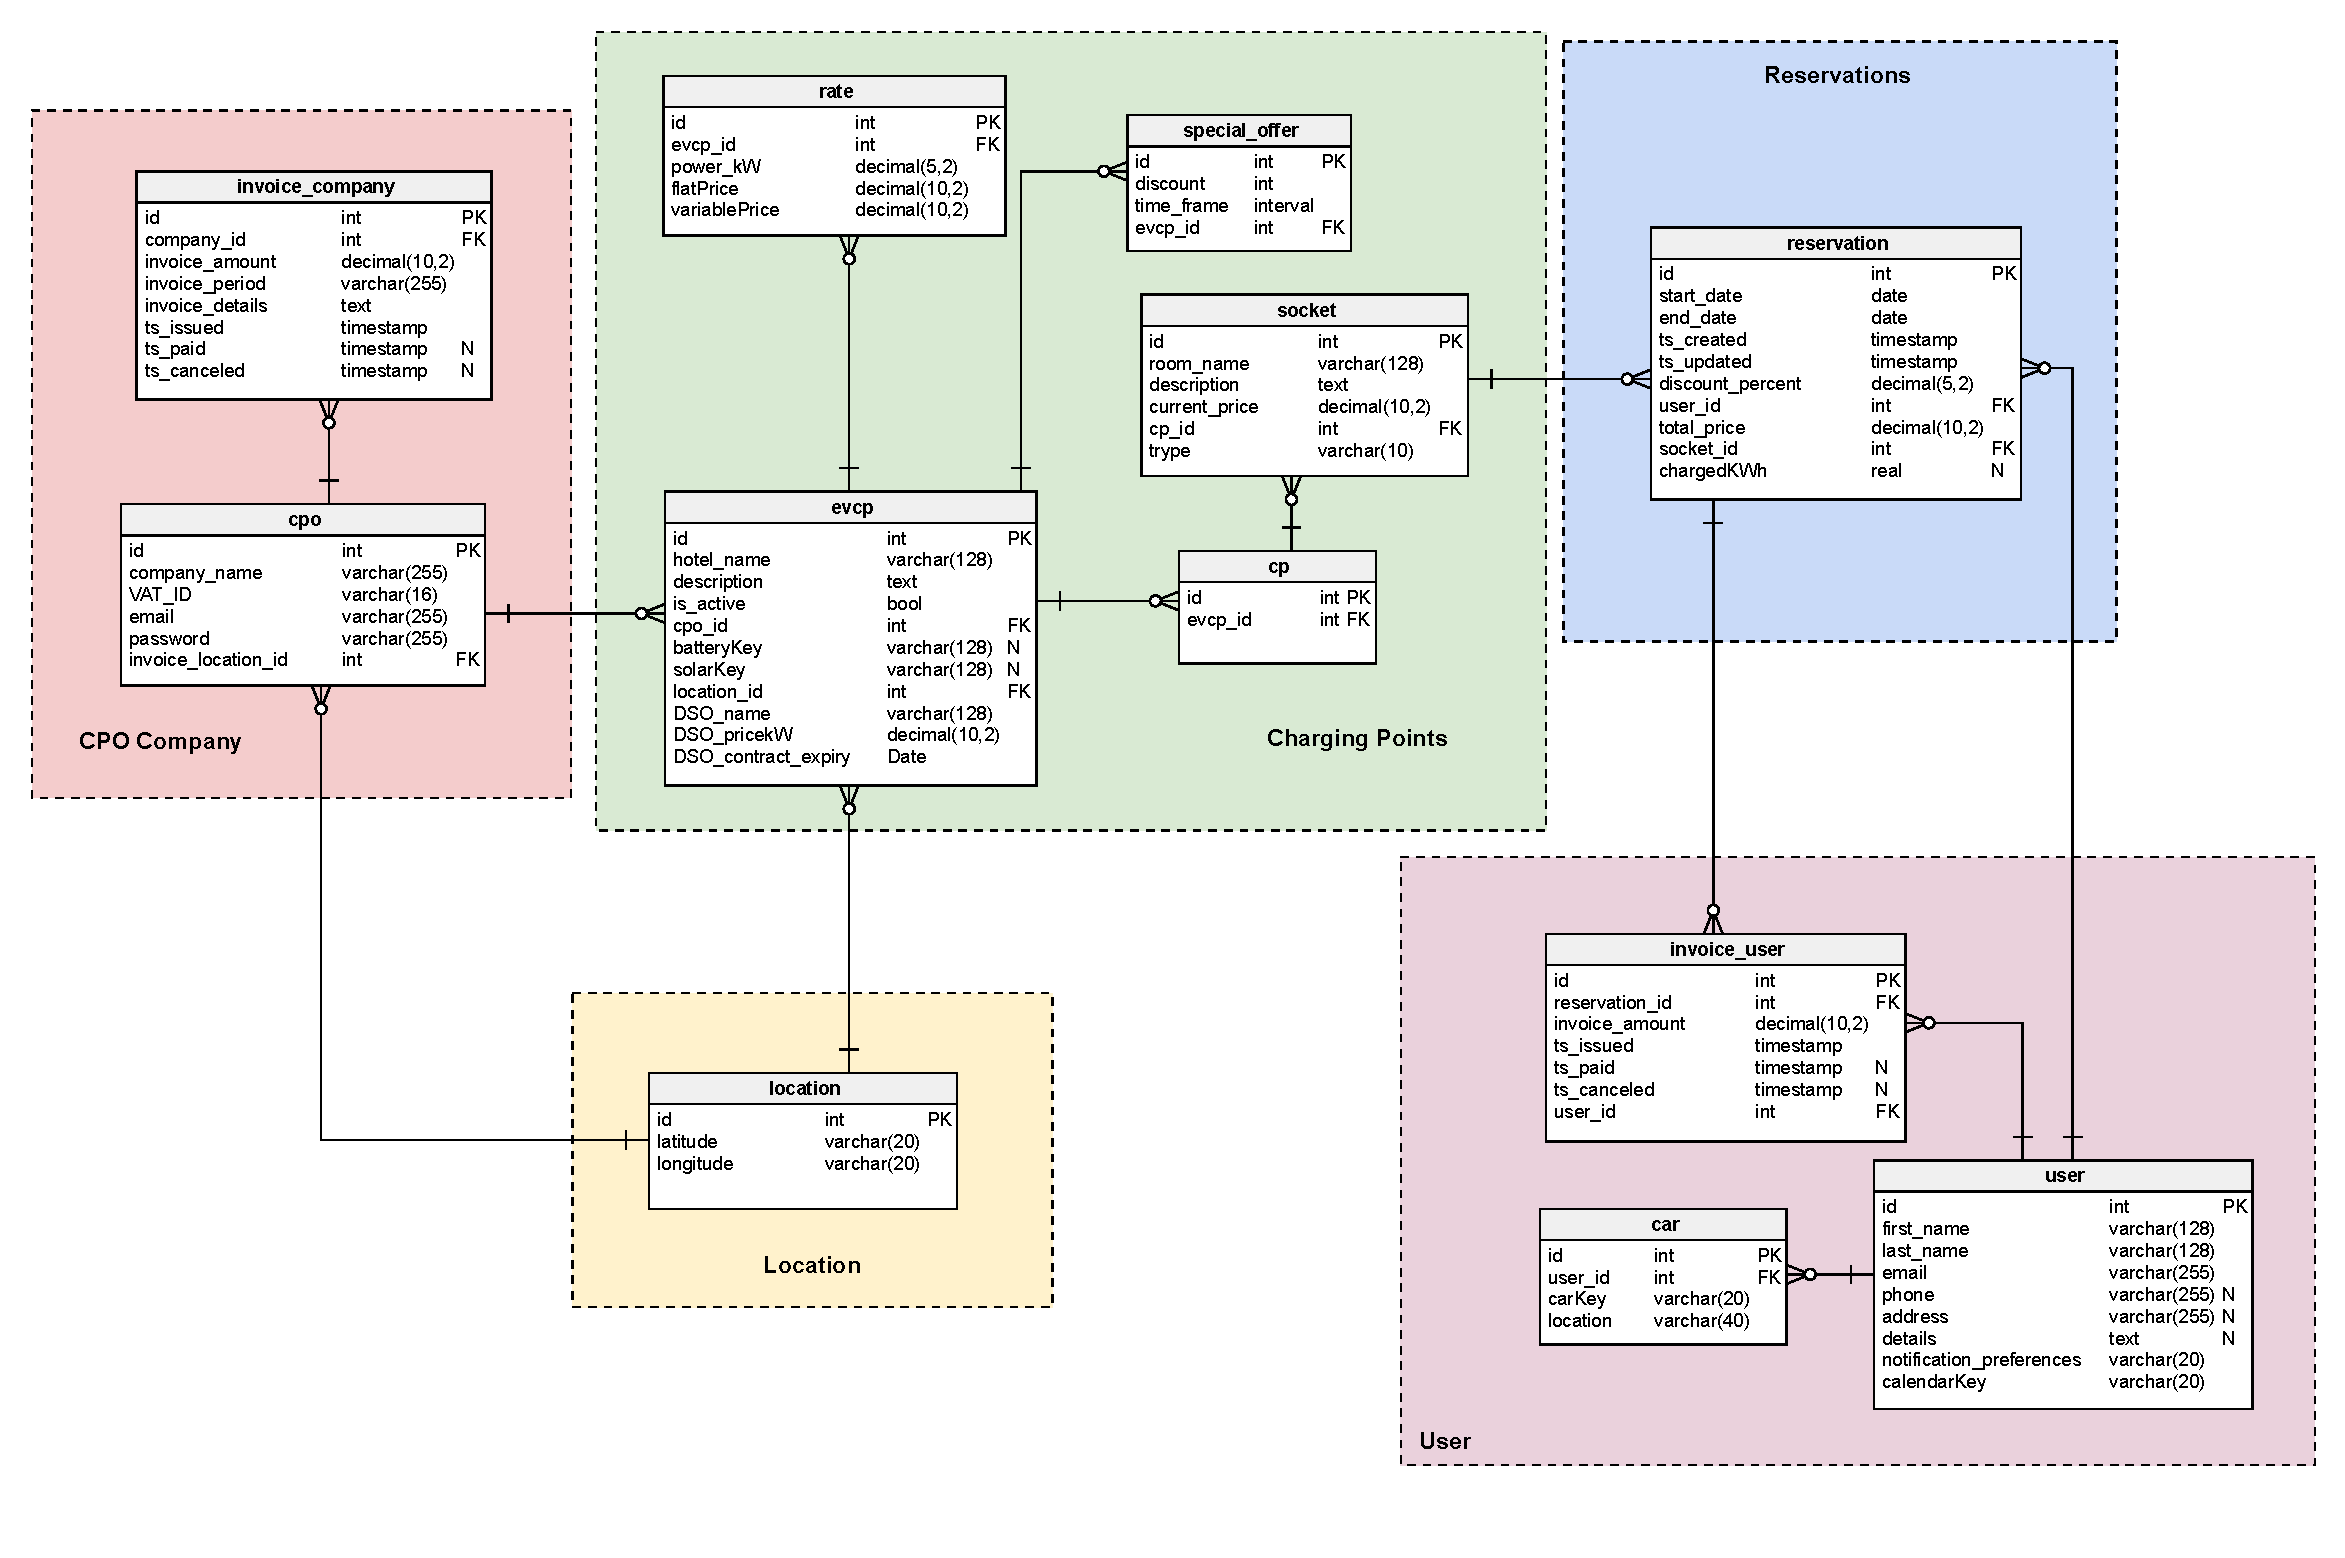
\includegraphics[scale=0.30]{src/ERDiagram/er_diagram.pdf}
\end{figure}

\subsection{Deployment view}
Infrastructure: deployment diagram(s) including non-logical elements (e.g., load balancer, firewall)

\subsection{Runtime view}
You can use sequence diagrams to describe the way components interact to accomplish specific tasks typically related to your use cases. Dynamics of the interactions: sequence
diagrams (realization of use cases)

\subsubsection{eMSP}
\begin{figure}[H]
    \centering
    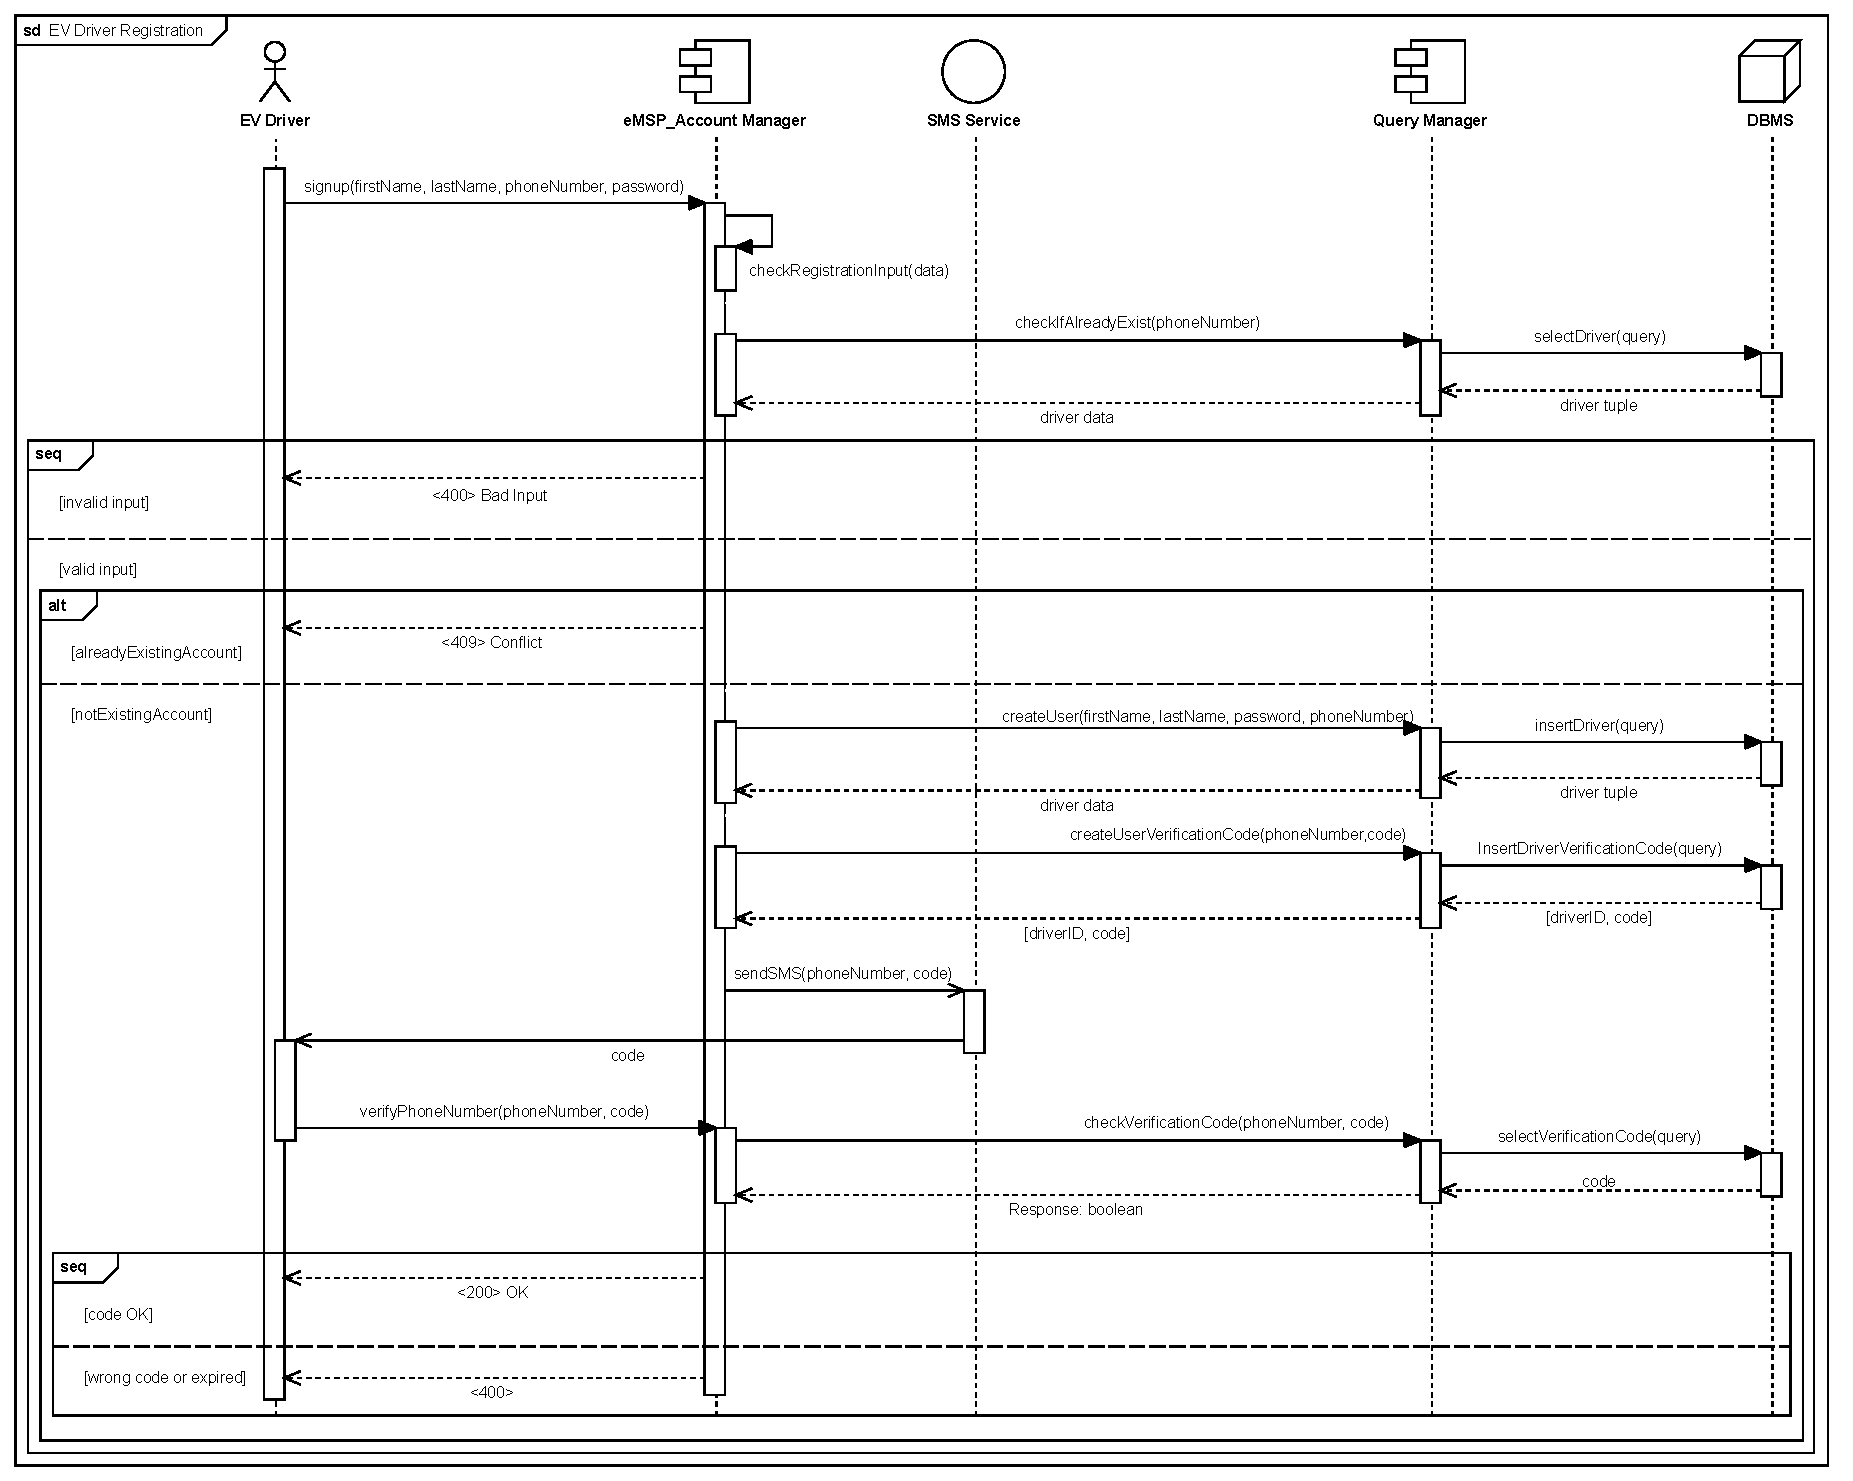
\includegraphics[scale=0.55]{src/runtimeVIew/eMSP_Registration.pdf}
    \caption{EV Driver Registration process}
\end{figure}

\begin{figure}[H]
    \centering
    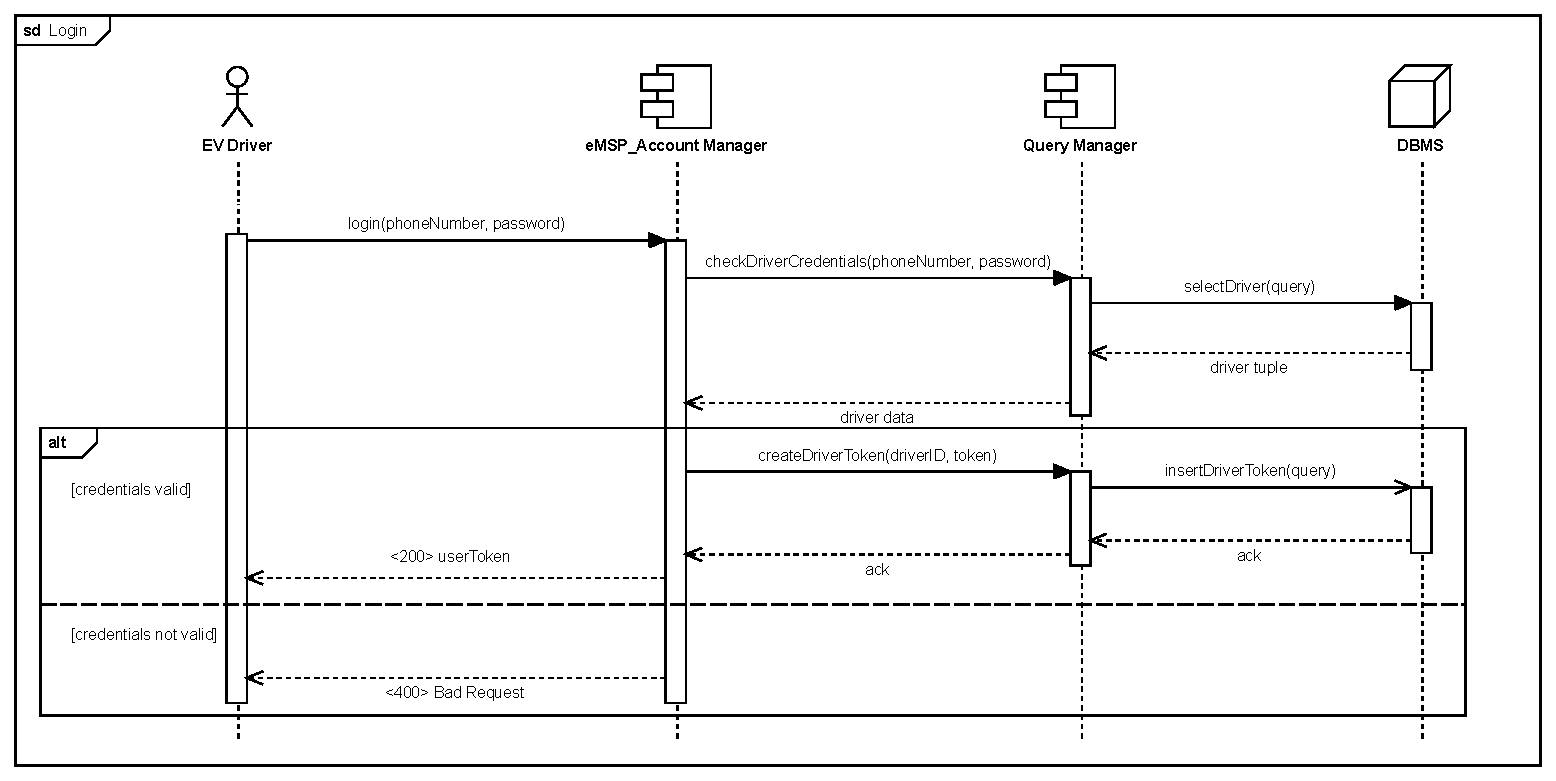
\includegraphics[scale=0.55]{src/runtimeVIew/eMSP_Login.pdf}
    \caption{EV Driver Logs in the system}
\end{figure}

\begin{figure}[H]
    \centering
    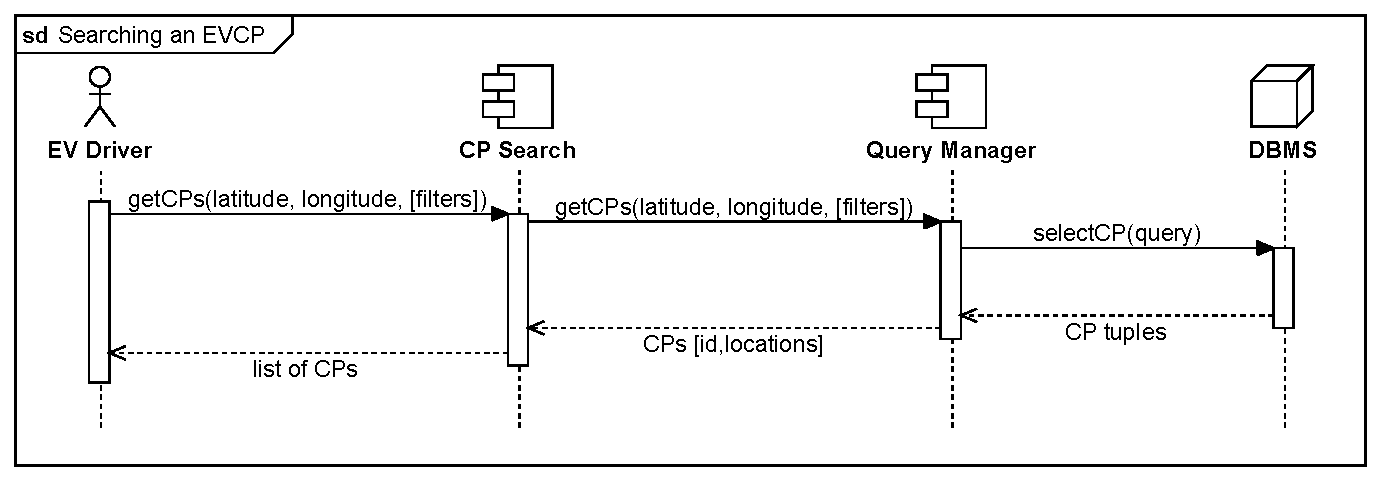
\includegraphics[scale=0.55]{src/runtimeVIew/eMSP_Search.pdf}
    \caption{EV Driver searches on the map}
\end{figure}

\begin{figure}[H]
    \centering
    \hspace*{-2cm}
    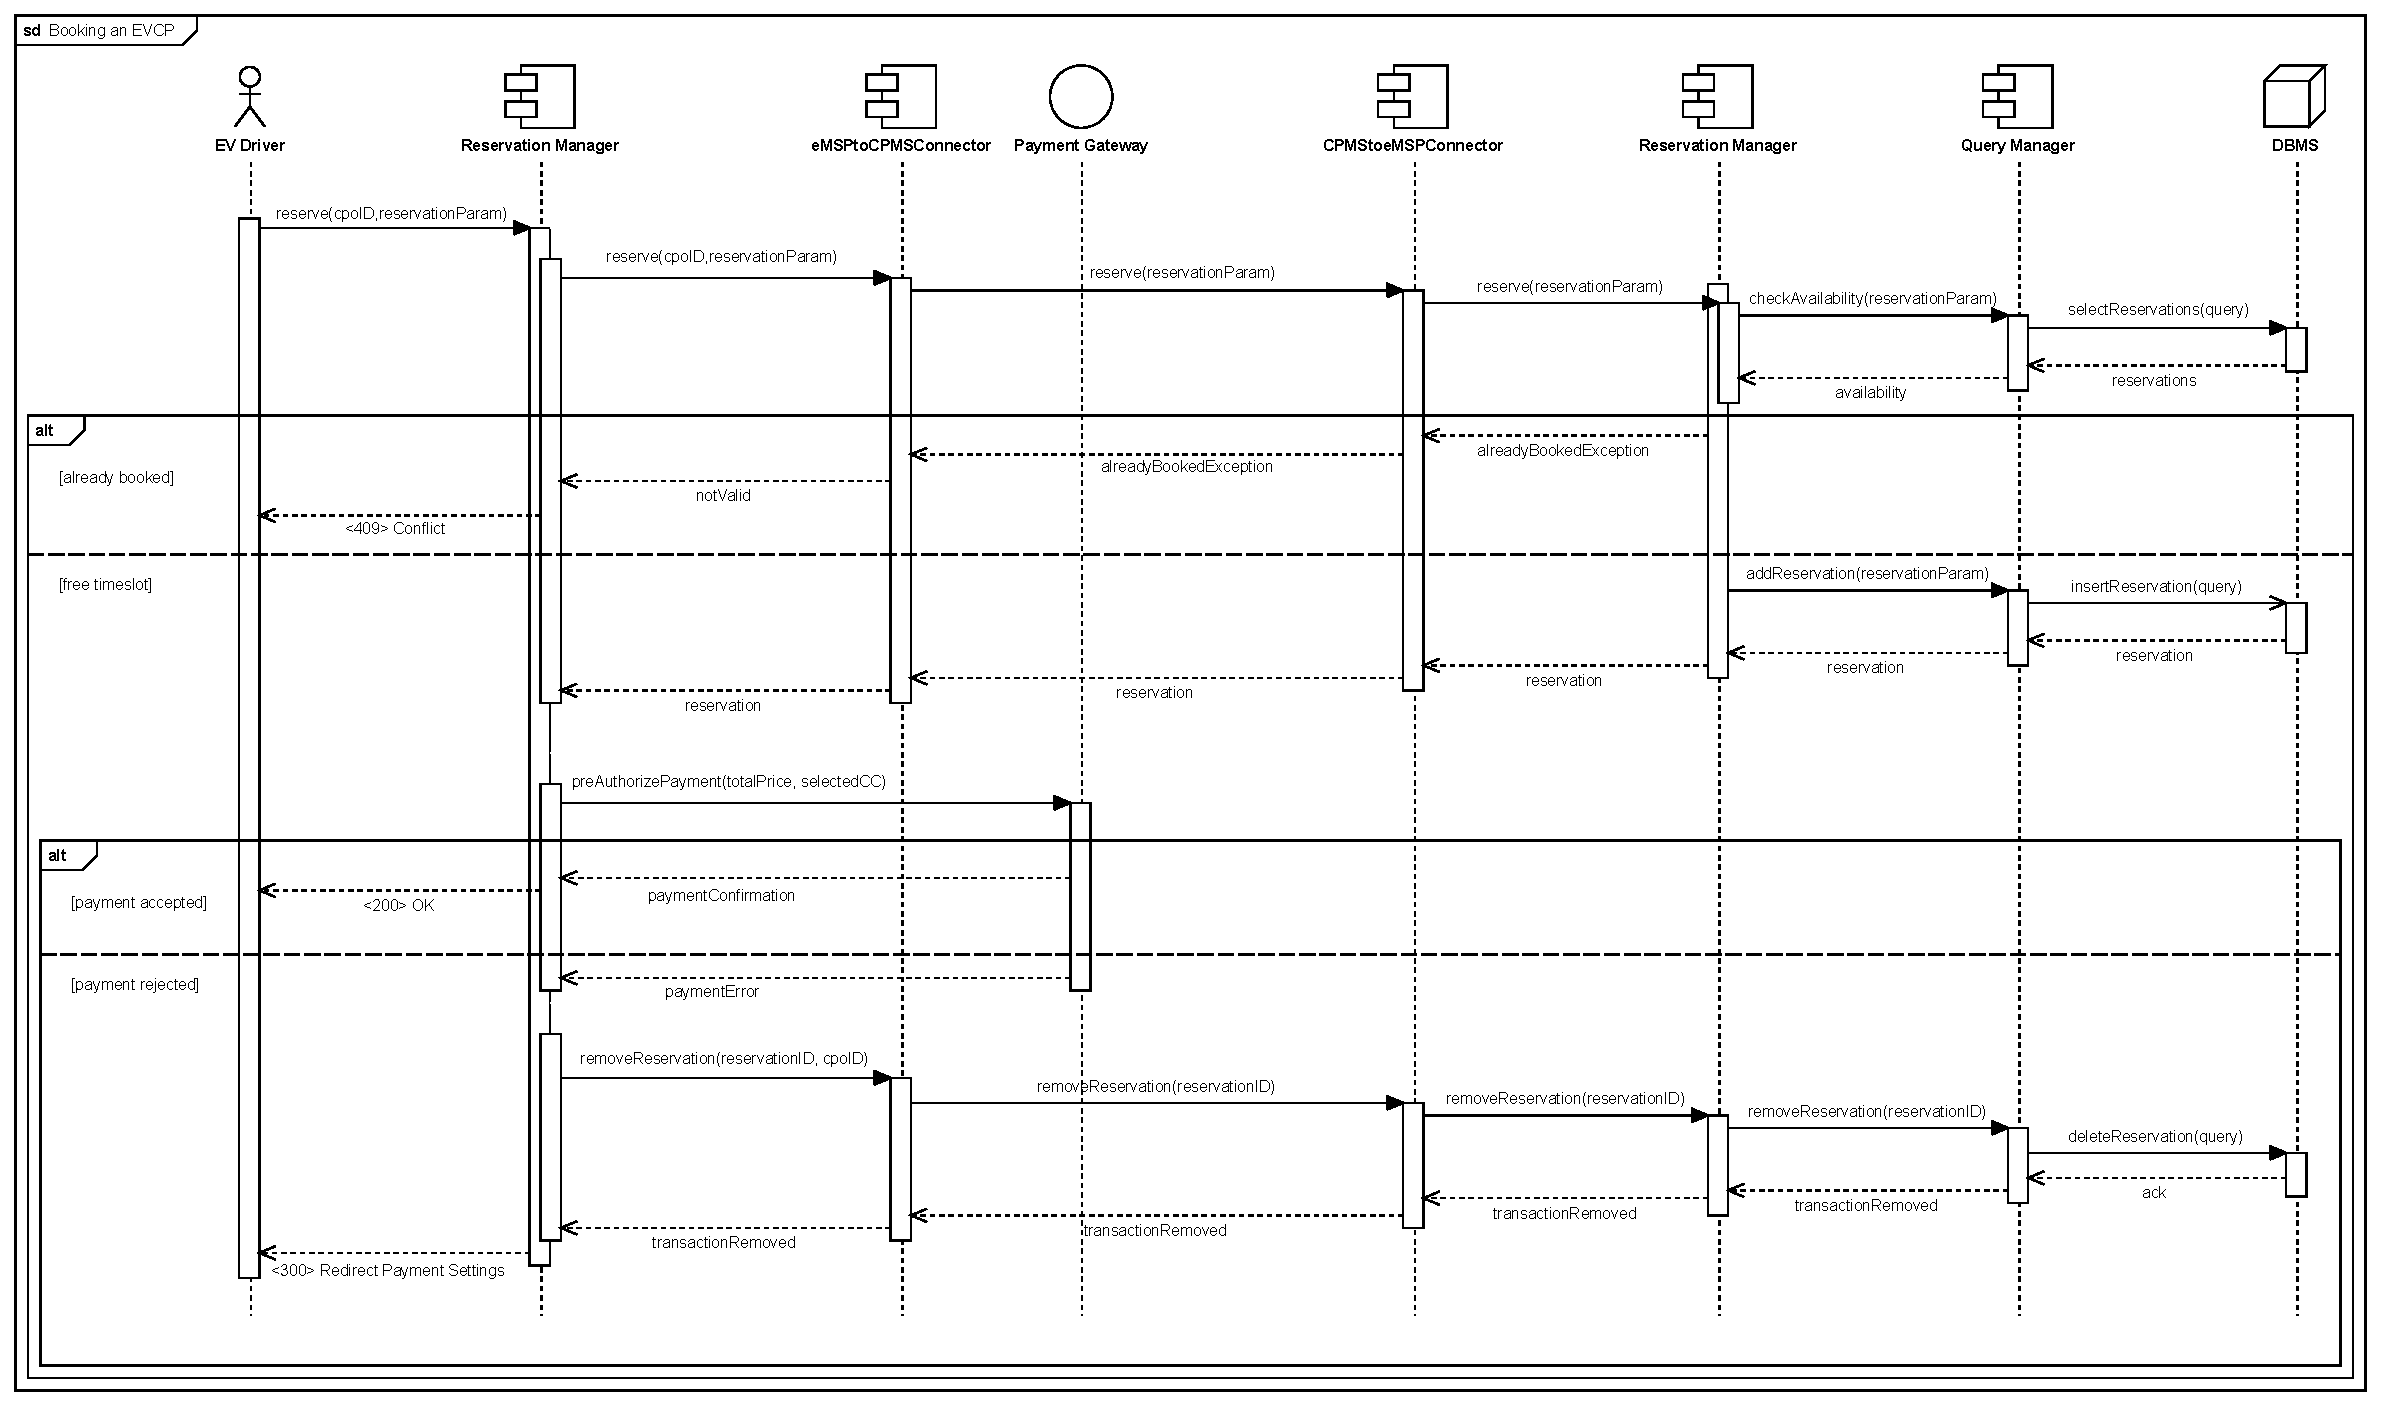
\includegraphics[scale=0.48]{src/runtimeVIew/eMSP_Book.pdf}
    \caption{EV Driver books a charge}
\end{figure}

\begin{figure}[H]
    \centering
    \hspace*{-2cm}
    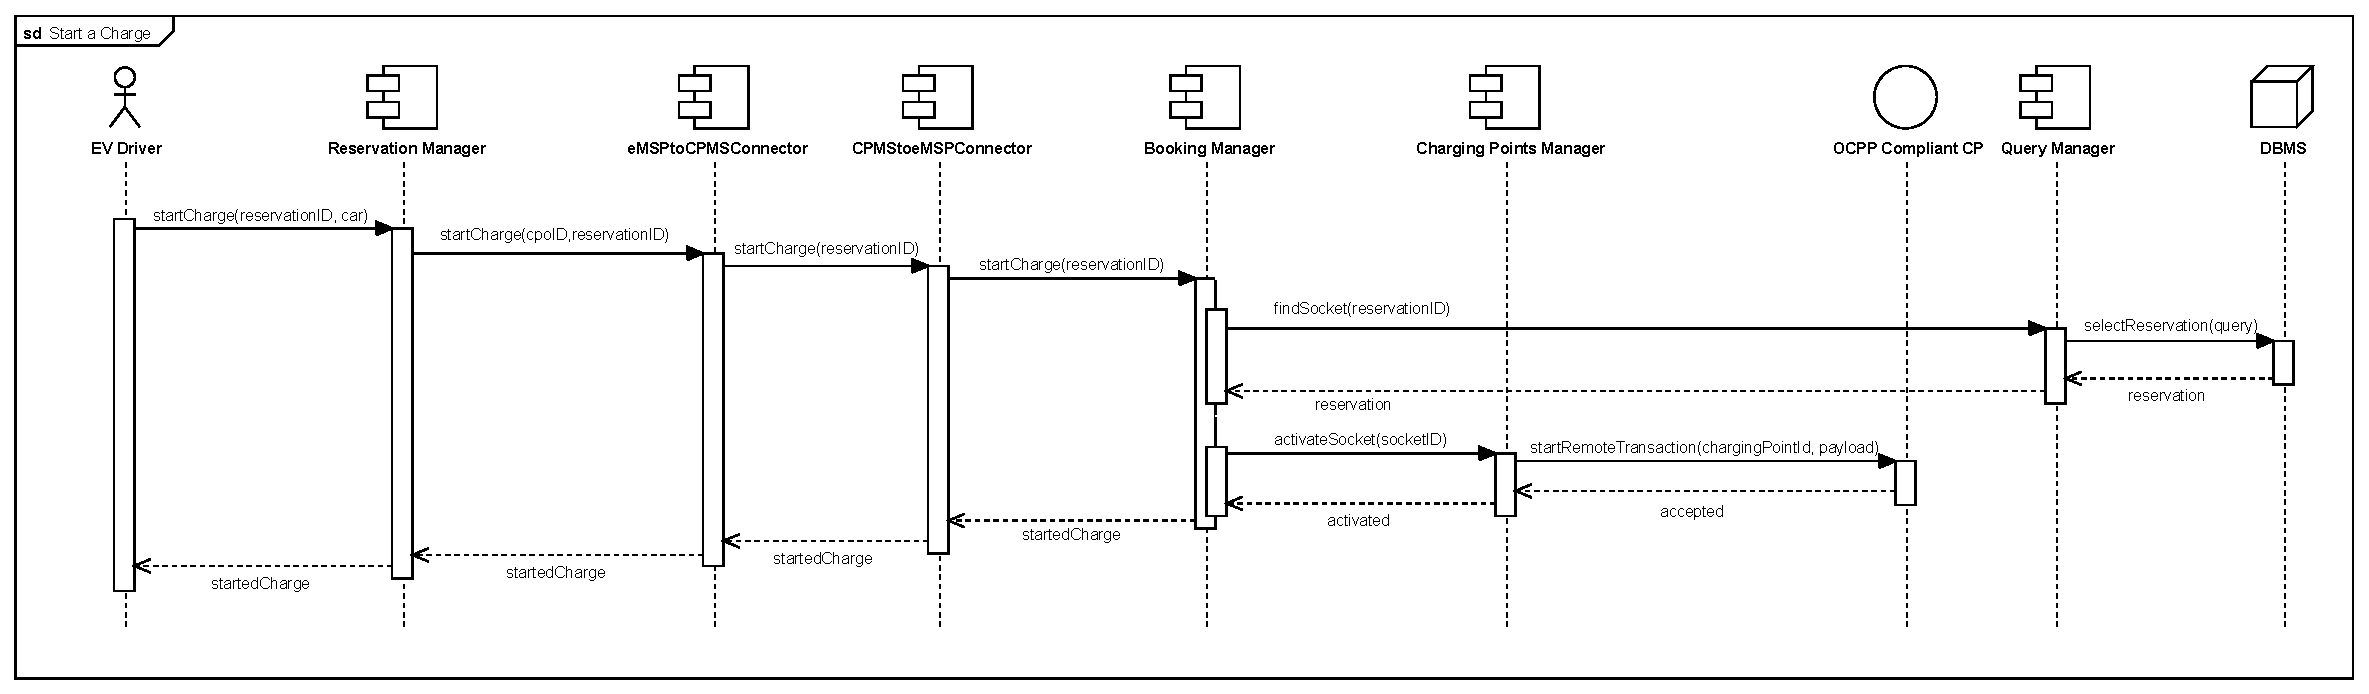
\includegraphics[scale=0.50]{src/runtimeVIew/eMSP_StartACharge.pdf}
    \caption{EV Driver starts a charge}
\end{figure}

\begin{figure}[H]
    \centering
    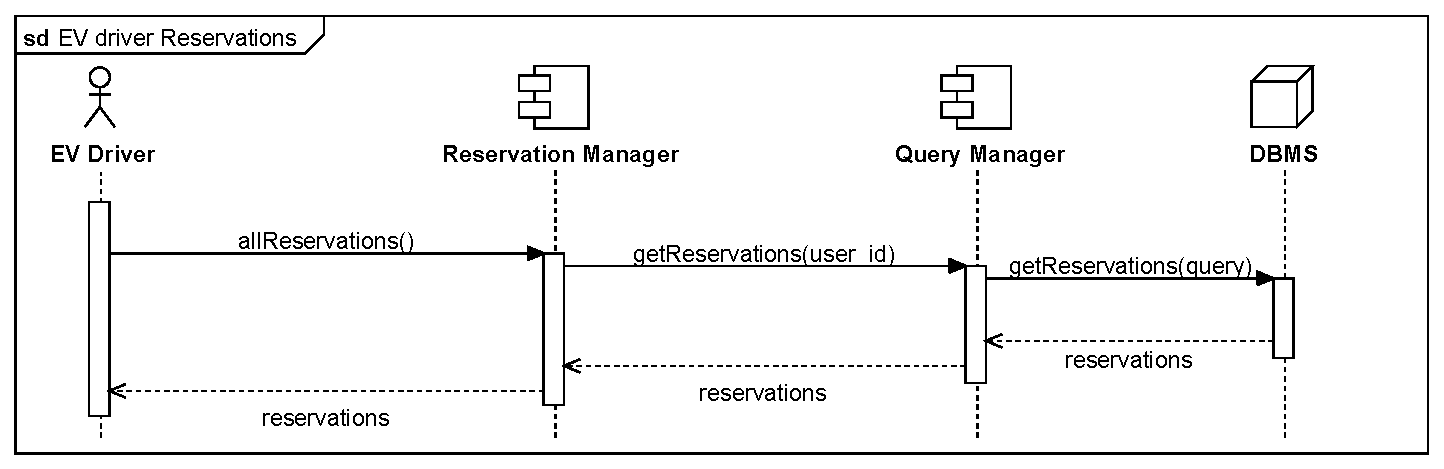
\includegraphics[scale=0.55]{src/runtimeVIew/eMSP_Reservations.pdf}
    \caption{EV Driver sees the reservations}
\end{figure}

\begin{figure}[H]
    \centering
    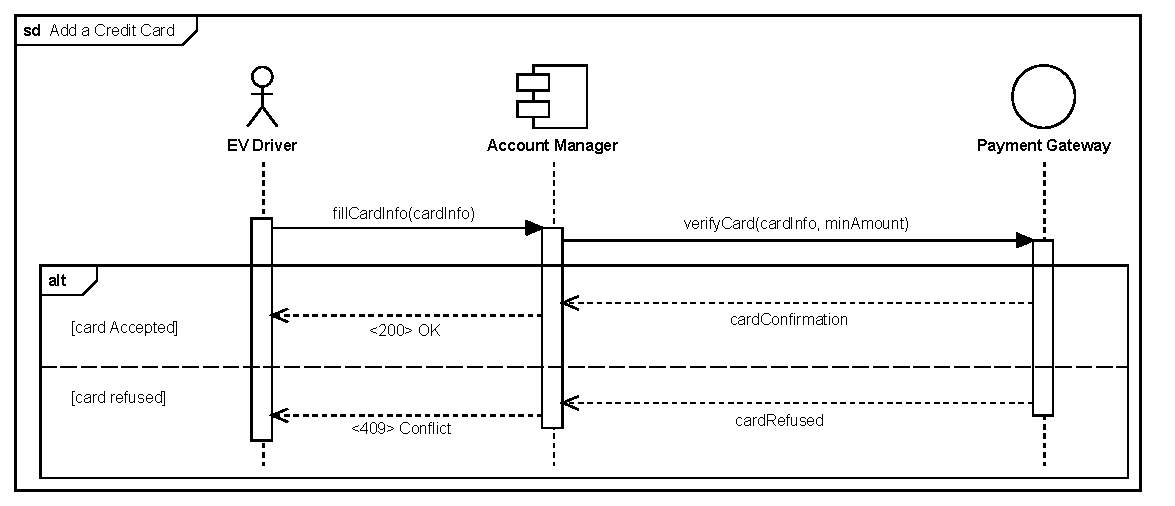
\includegraphics[scale=0.55]{src/runtimeVIew/eMSP_AddCC.pdf}
    \caption{EV Driver adds a credit card information}
\end{figure}

\subsubsection{CPMS}
\begin{figure}[H]
    \centering
    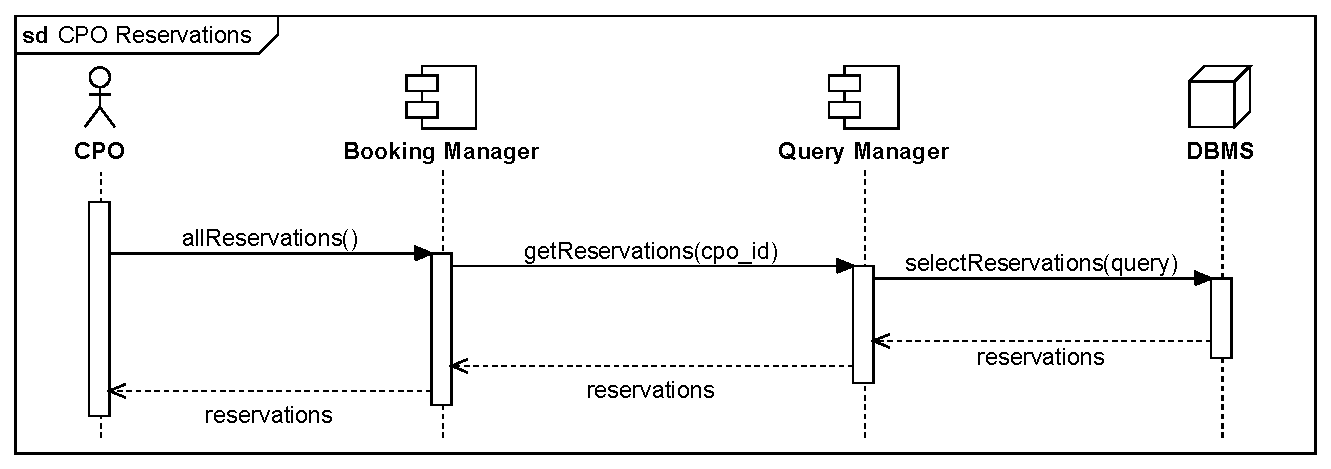
\includegraphics[scale=0.55]{src/runtimeVIew/CPMS_Reservations.pdf}
    \caption{CPO sees the reservations}
\end{figure}

\begin{figure}[H]
    \centering
    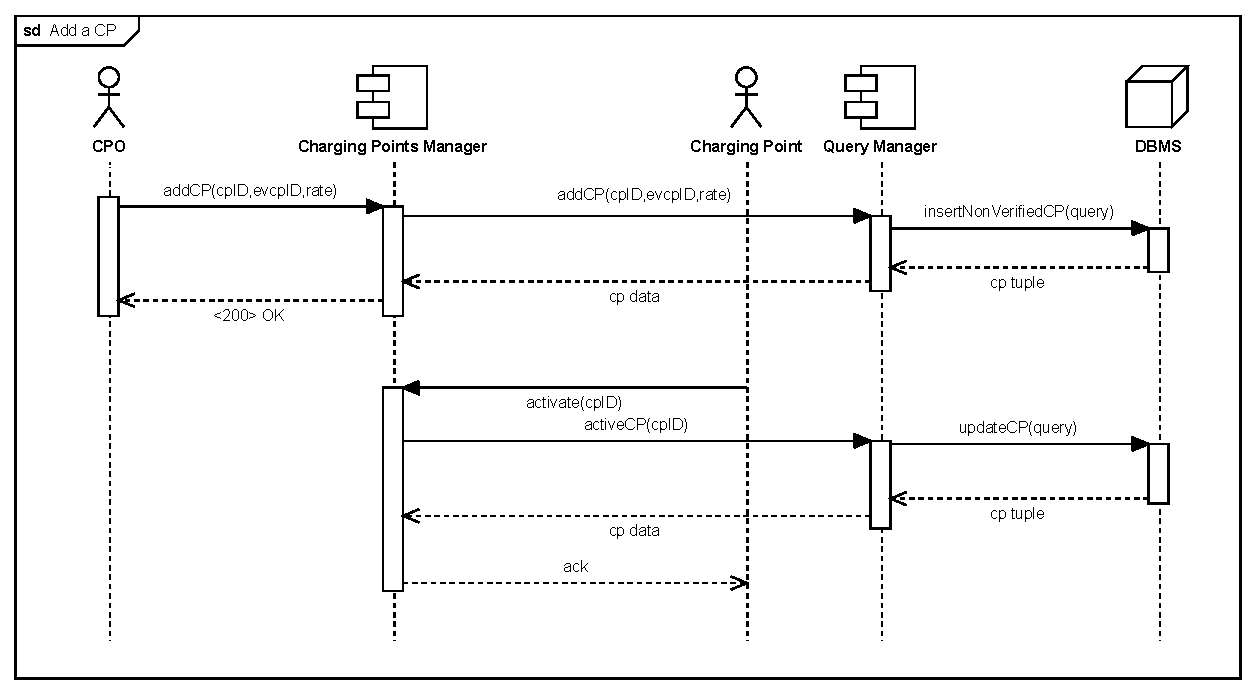
\includegraphics[scale=0.55]{src/runtimeVIew/CPMS_AddCP.pdf}
    \caption{CPO adds a Charging Point}
\end{figure}

\begin{figure}[H]
    \centering
    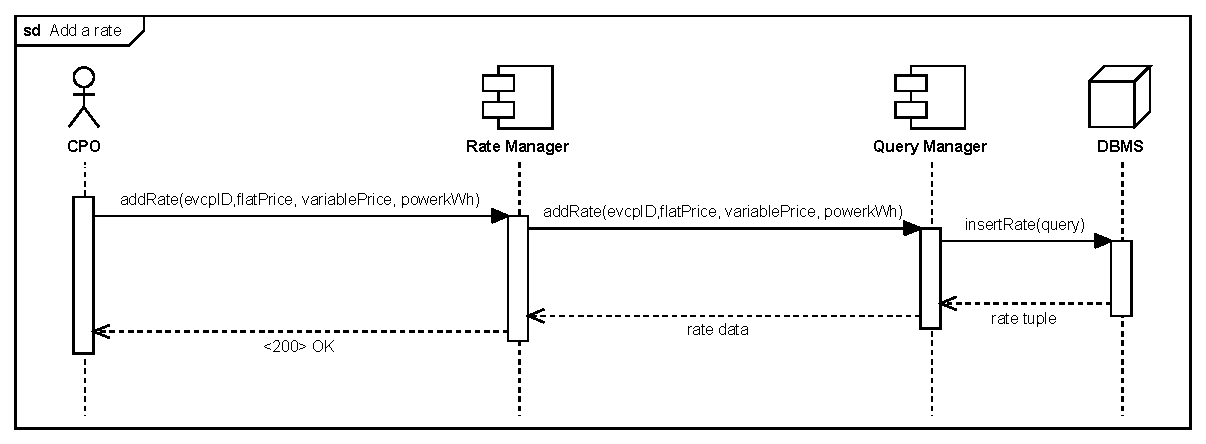
\includegraphics[scale=0.55]{src/runtimeVIew/CPMS_addRate.pdf}
    \caption{CPO adds a rate}
\end{figure}

\begin{figure}[H]
    \centering
    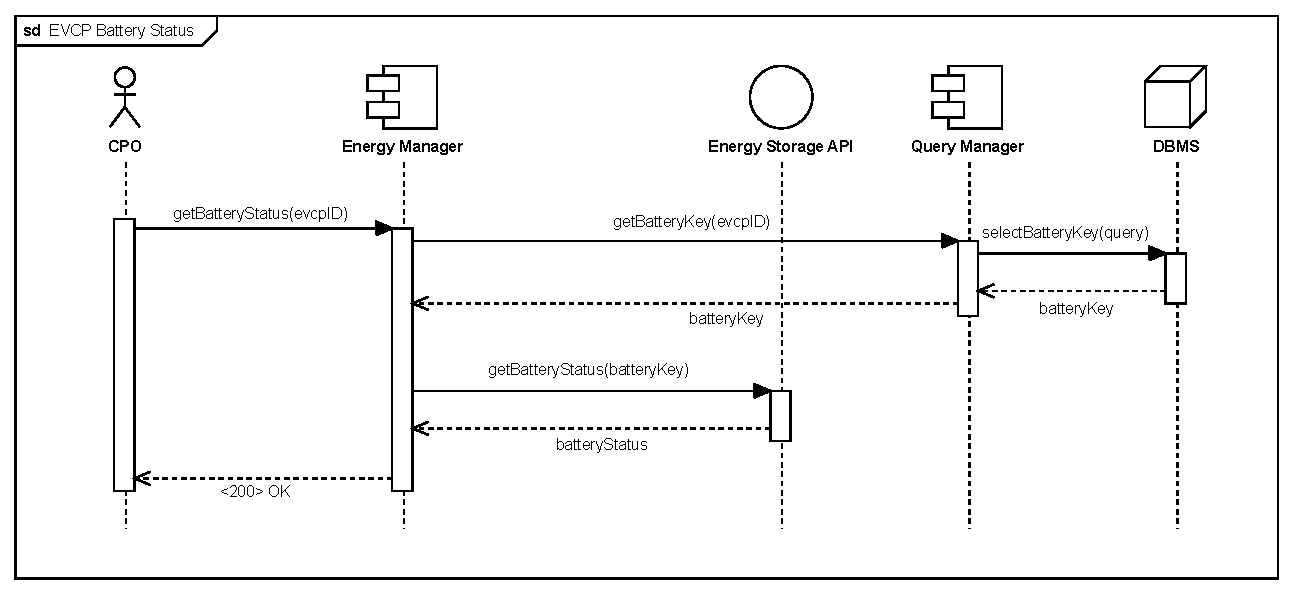
\includegraphics[scale=0.55]{src/runtimeVIew/CPMS_batteryCapacity.pdf}
    \caption{CPO sees the battery capacity}
\end{figure}

\begin{figure}[H]
    \centering
    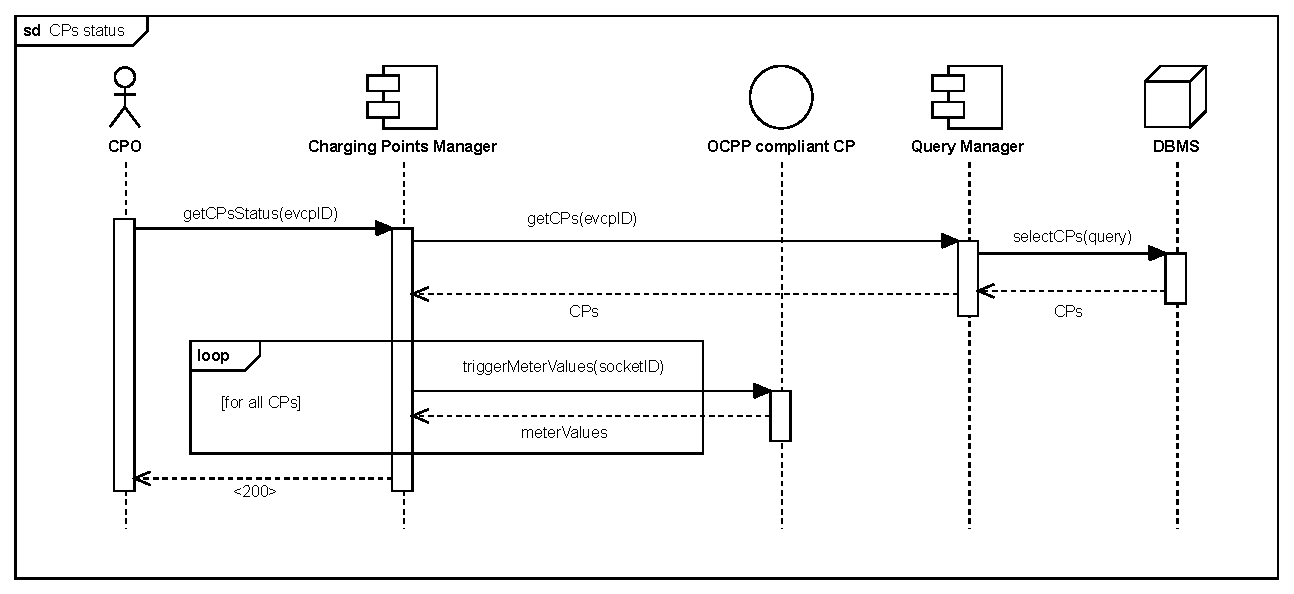
\includegraphics[scale=0.55]{src/runtimeVIew/CPMS_CPsStatus.pdf}
    \caption{CPO sees the status of its Charging Points}
\end{figure}

\begin{figure}[H]
    \centering
    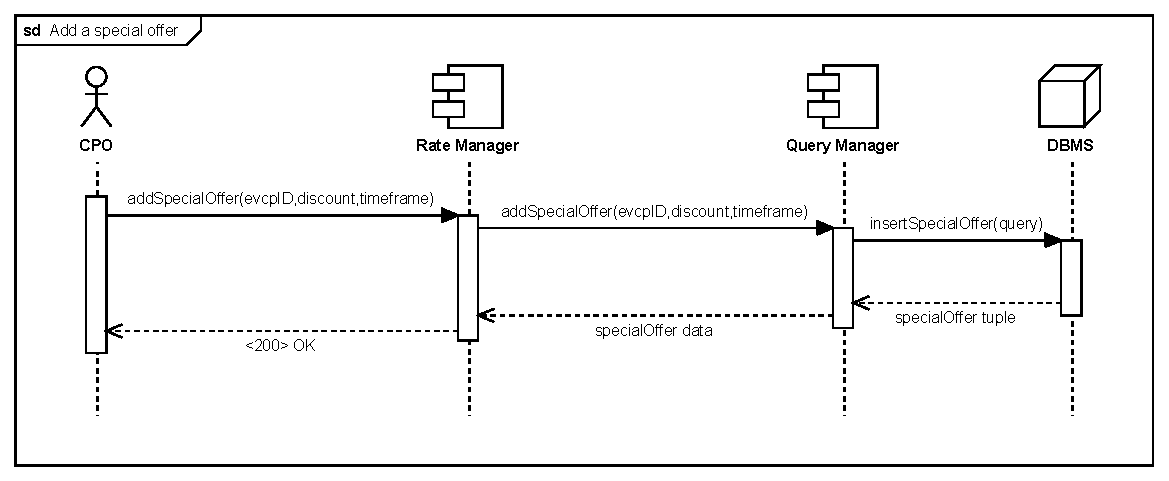
\includegraphics[scale=0.55]{src/runtimeVIew/CPMS_specialOffer.pdf}
    \caption{CPO adds a special offer}
\end{figure}

\subsection{Component interfaces}
Details for each interface (name, signature, returned objects)
\subsubsection{REST Endpoints}
\renewcommand{\labelitemii}{}
\renewcommand{\labelitemiii}{-}
\begin{itemize}
    \item \texttt{/api/search/<latitude|longitude>}
          \begin{itemize}
              \item Maps: \texttt{NomeMetodoMappato}
              \item Type: TipoAPI(GET,POST)
              \item URL Parameters:
                    \begin{itemize}
                        \item \texttt{<latitude|longitude>} - GPS Location, needed to find CPs nearby a certain location.
                    \end{itemize}
              \item Parameters:
                    \begin{itemize}
                        \item \texttt{authToken}
                        \item \texttt{blabla} [string] - description
                        \item \texttt{blabla} [boolean] - description
                        \item \texttt{blabla} [number] - description
                    \end{itemize}
              \item Success:
                    \begin{itemize}
                        \item 200 - OK + Response
                              \begin{lstlisting}
            {
                "cps": [
                    {
                        "id": "<store id>",
                        "name": "<cp name>",
                        "address": "<address>",
                        "open": <boolean>,
                        "distance": <number>,
                    }
                ]
            }
            \end{lstlisting}
                    \end{itemize}
              \item Errors:
                    \begin{itemize}
                        \item 400 - Bad request
                        \item 404 - No store found
                    \end{itemize}
          \end{itemize}
\end{itemize}

\subsection{Architectural Styles and patterns}
Please explain which styles/patterns you used, why, and how

\begin{itemize}
    \item Three layers and Four Tier: what and why?
    \item RESTful: what and why?
    \item Adapter Pattern: The Query Manager component implements the Adapter pattern, as it mediates between the
          business logic and the DBMS services, exposing only a restricted and higher level set of functionalities.
\end{itemize}
\subsection{Other design decisions}
\subsubsection{PWA}
\dots
\subsubsection{Scale-out}
\dots
\subsubsection{Relational Database}
\dots
\subsubsection{The separation of eMSP and CPMSs}